%DIF 1-6d1
%DIF LATEXDIFF DIFFERENCE FILE
%DIF DEL C:\Users\Simon\OneDrive - BTH\Research\Weed\Articel\Access\IEEE_Access_before_review\access_revised_v2.tex         Fri Apr 10 00:40:30 2026
%DIF ADD C:\Users\Simon\OneDrive - BTH\Research\Weed\Articel\Access\WeedArticleI_IEEE_Access__Copy_\access_revised_v2.tex   Wed Apr 22 19:54:48 2026
%DIF < 
%DIF < 
%DIF < \usepackage{float}
%DIF < 
%DIF < 
%DIF < 
%DIF -------
\documentclass{ieeeaccess}
%DIF 8a2
\usepackage{float} %DIF > 
%DIF -------
\usepackage{cite}
\usepackage{amsmath,amssymb,amsfonts}
\usepackage{algorithmic}
\usepackage{graphicx}
\usepackage{textcomp}


\usepackage{bm}
\makeatletter
\AtBeginDocument{\DeclareMathVersion{bold}
\SetSymbolFont{operators}{bold}{T1}{times}{b}{n}
%DIF 19c14
%DIF < \SetSymbolFont{NewLetters}{bold}{T1}{times}{b}{it}
%DIF -------
\SetSymbolFont{letters}{bold}{T1}{times}{b}{it} %DIF > 
%DIF -------
\SetMathAlphabet{\mathrm}{bold}{T1}{times}{b}{n}
\SetMathAlphabet{\mathit}{bold}{T1}{times}{b}{it}
\SetMathAlphabet{\mathbf}{bold}{T1}{times}{b}{n}
\SetMathAlphabet{\mathtt}{bold}{OT1}{pcr}{b}{n}
\SetSymbolFont{symbols}{bold}{OMS}{cmsy}{b}{n}
\renewcommand\boldmath{\@nomath\boldmath\mathversion{bold}}}
\makeatother

\usepackage{booktabs}

\def\BibTeX{{\rm B\kern-.05em{\sc i\kern-.025em b}\kern-.08em
    T\kern-.1667em\lower.7ex\hbox{E}\kern-.125emX}}



\usepackage{subfigure} % Add this package
 %DIF > 
\providecommand{\xfigwd}{0pt} %DIF > 
%DIF PREAMBLE EXTENSION ADDED BY LATEXDIFF
%DIF UNDERLINE PREAMBLE %DIF PREAMBLE
\RequirePackage[normalem]{ulem} %DIF PREAMBLE
\RequirePackage{color}\definecolor{RED}{rgb}{1,0,0}\definecolor{BLUE}{rgb}{0,0,1} %DIF PREAMBLE
\providecommand{\DIFadd}[1]{{\protect\color{blue}\uwave{#1}}} %DIF PREAMBLE
\providecommand{\DIFdel}[1]{{\protect\color{red}\sout{#1}}} %DIF PREAMBLE
%DIF SAFE PREAMBLE %DIF PREAMBLE
\providecommand{\DIFaddbegin}{} %DIF PREAMBLE
\providecommand{\DIFaddend}{} %DIF PREAMBLE
\providecommand{\DIFdelbegin}{} %DIF PREAMBLE
\providecommand{\DIFdelend}{} %DIF PREAMBLE
\providecommand{\DIFmodbegin}{} %DIF PREAMBLE
\providecommand{\DIFmodend}{} %DIF PREAMBLE
%DIF FLOATSAFE PREAMBLE %DIF PREAMBLE
\providecommand{\DIFaddFL}[1]{\DIFadd{#1}} %DIF PREAMBLE
\providecommand{\DIFdelFL}[1]{\DIFdel{#1}} %DIF PREAMBLE
\providecommand{\DIFaddbeginFL}{} %DIF PREAMBLE
\providecommand{\DIFaddendFL}{} %DIF PREAMBLE
\providecommand{\DIFdelbeginFL}{} %DIF PREAMBLE
\providecommand{\DIFdelendFL}{} %DIF PREAMBLE
\providecommand{\DIFscaledelfig}{0.5}
%DIF HIGHLIGHTGRAPHICS PREAMBLE %DIF PREAMBLE
\RequirePackage{settobox} %DIF PREAMBLE
\RequirePackage{letltxmacro} %DIF PREAMBLE
\newsavebox{\DIFdelgraphicsbox} %DIF PREAMBLE
\newlength{\DIFdelgraphicswidth} %DIF PREAMBLE
\newlength{\DIFdelgraphicsheight} %DIF PREAMBLE
% store original definition of \includegraphics %DIF PREAMBLE
\LetLtxMacro{\DIFOincludegraphics}{\includegraphics} %DIF PREAMBLE
\providecommand{\DIFaddincludegraphics}[2][]{{\color{blue}\fbox{\DIFOincludegraphics[#1]{#2}}}} %DIF PREAMBLE
\providecommand{\DIFdelincludegraphics}[2][]{% %DIF PREAMBLE
\sbox{\DIFdelgraphicsbox}{\DIFOincludegraphics[#1]{#2}}% %DIF PREAMBLE
\settoboxwidth{\DIFdelgraphicswidth}{\DIFdelgraphicsbox} %DIF PREAMBLE
\settoboxtotalheight{\DIFdelgraphicsheight}{\DIFdelgraphicsbox} %DIF PREAMBLE
\scalebox{\DIFscaledelfig}{% %DIF PREAMBLE
\parbox[b]{\DIFdelgraphicswidth}{\usebox{\DIFdelgraphicsbox}\\[-\baselineskip] \rule{\DIFdelgraphicswidth}{0em}}\llap{\resizebox{\DIFdelgraphicswidth}{\DIFdelgraphicsheight}{% %DIF PREAMBLE
\setlength{\unitlength}{\DIFdelgraphicswidth}% %DIF PREAMBLE
\begin{picture}(1,1)% %DIF PREAMBLE
\thicklines\linethickness{2pt} %DIF PREAMBLE
{\color[rgb]{1,0,0}\put(0,0){\framebox(1,1){}}}% %DIF PREAMBLE
{\color[rgb]{1,0,0}\put(0,0){\line( 1,1){1}}}% %DIF PREAMBLE
{\color[rgb]{1,0,0}\put(0,1){\line(1,-1){1}}}% %DIF PREAMBLE
\end{picture}% %DIF PREAMBLE
}\hspace*{3pt}}} %DIF PREAMBLE
} %DIF PREAMBLE
\LetLtxMacro{\DIFOaddbegin}{\DIFaddbegin} %DIF PREAMBLE
\LetLtxMacro{\DIFOaddend}{\DIFaddend} %DIF PREAMBLE
\LetLtxMacro{\DIFOdelbegin}{\DIFdelbegin} %DIF PREAMBLE
\LetLtxMacro{\DIFOdelend}{\DIFdelend} %DIF PREAMBLE
\DeclareRobustCommand{\DIFaddbegin}{\DIFOaddbegin \let\includegraphics\DIFaddincludegraphics} %DIF PREAMBLE
\DeclareRobustCommand{\DIFaddend}{\DIFOaddend \let\includegraphics\DIFOincludegraphics} %DIF PREAMBLE
\DeclareRobustCommand{\DIFdelbegin}{\DIFOdelbegin \let\includegraphics\DIFdelincludegraphics} %DIF PREAMBLE
\DeclareRobustCommand{\DIFdelend}{\DIFOaddend \let\includegraphics\DIFOincludegraphics} %DIF PREAMBLE
\LetLtxMacro{\DIFOaddbeginFL}{\DIFaddbeginFL} %DIF PREAMBLE
\LetLtxMacro{\DIFOaddendFL}{\DIFaddendFL} %DIF PREAMBLE
\LetLtxMacro{\DIFOdelbeginFL}{\DIFdelbeginFL} %DIF PREAMBLE
\LetLtxMacro{\DIFOdelendFL}{\DIFdelendFL} %DIF PREAMBLE
\DeclareRobustCommand{\DIFaddbeginFL}{\DIFOaddbeginFL \let\includegraphics\DIFaddincludegraphics} %DIF PREAMBLE
\DeclareRobustCommand{\DIFaddendFL}{\DIFOaddendFL \let\includegraphics\DIFOincludegraphics} %DIF PREAMBLE
\DeclareRobustCommand{\DIFdelbeginFL}{\DIFOdelbeginFL \let\includegraphics\DIFdelincludegraphics} %DIF PREAMBLE
\DeclareRobustCommand{\DIFdelendFL}{\DIFOaddendFL \let\includegraphics\DIFOincludegraphics} %DIF PREAMBLE
%DIF AMSMATHULEM PREAMBLE %DIF PREAMBLE
\makeatletter %DIF PREAMBLE
\let\sout@orig\sout %DIF PREAMBLE
\renewcommand{\sout}[1]{\ifmmode\text{\sout@orig{\ensuremath{#1}}}\else\sout@orig{#1}\fi} %DIF PREAMBLE
\makeatother %DIF PREAMBLE
%DIF COLORLISTINGS PREAMBLE %DIF PREAMBLE
\RequirePackage{listings} %DIF PREAMBLE
\RequirePackage{color} %DIF PREAMBLE
\lstdefinelanguage{DIFcode}{ %DIF PREAMBLE
%DIF DIFCODE_UNDERLINE %DIF PREAMBLE
  moredelim=[il][\color{red}\sout]{\%DIF\ <\ }, %DIF PREAMBLE
  moredelim=[il][\color{blue}\uwave]{\%DIF\ >\ } %DIF PREAMBLE
} %DIF PREAMBLE
\lstdefinestyle{DIFverbatimstyle}{ %DIF PREAMBLE
	language=DIFcode, %DIF PREAMBLE
	basicstyle=\ttfamily, %DIF PREAMBLE
	columns=fullflexible, %DIF PREAMBLE
	keepspaces=true %DIF PREAMBLE
} %DIF PREAMBLE
\lstnewenvironment{DIFverbatim}[1][]{\lstset{style=DIFverbatimstyle}}{} %DIF PREAMBLE
\lstnewenvironment{DIFverbatim*}[1][]{\lstset{style=DIFverbatimstyle,showspaces=true}}{} %DIF PREAMBLE
\lstset{extendedchars=\true,inputencoding=utf8}

%DIF END PREAMBLE EXTENSION ADDED BY LATEXDIFF

\begin{document}
\history{Date of publication xxxx 00, 0000, date of current version xxxx 00, 0000.}
%DIF <  \doi{10.1109/ACCESS.2017.DOI}
\DIFaddbegin \doi{10.1109/ACCESS.2017.DOI}
\DIFaddend 



\title{Impact of Multispectral Imaging and Vegetation Indices on Neural Network Performance for Weed Detection Using Agricultural UAVs}


\author{\uppercase{Simon Hallösta}
\authorrefmark{1}
, 
\uppercase{Saleh Javadi}
\authorrefmark{1}
, 
\uppercase{Mattias Dahl}
\authorrefmark{1}
,
\uppercase{Mats I. Pettersson}
\authorrefmark{1}
}


\address[1]{Department of Mathematics and Natural Sciences, Blekinge Institute of Technology, 371 79 Karlskrona, Sweden}


\markboth
{Hallösta \headeretal: Multispectral VIs for UAV Weed Detection}
{Hallösta \headeretal: Multispectral VIs for UAV Weed Detection}

\corresp{Corresponding author: Simon Hallösta (e-mail: simon.hallosta@bth.se).}



\begin{abstract}




The integration of multispectral imaging data with vegetation indices (VIs) offers potential improvements in weed detection for precision agriculture. Weed detection, particularly for species like black-grass (\textit{Alopecurus myosuroides}), remains challenging due to its visual similarity to crops like wheat\DIFaddbegin \DIFadd{, especially during the limited spring period in which the weed is both observable and still relevant for control}\DIFaddend . By utilizing data captured from unmanned aerial vehicles (UAVs) over winter wheat fields, we assess the impact of key \DIFdelbegin \DIFdel{VIs—including }\DIFdelend \DIFaddbegin \DIFadd{VIs--including }\DIFaddend the Normalized Difference Vegetation Index (NDVI), Triangular Greenness Index (TGI), and Excess Green Index (ExG)\DIFdelbegin \DIFdel{—on }\DIFdelend \DIFaddbegin \DIFadd{--on }\DIFaddend the accuracy of black-grass detection. A \DIFdelbegin \DIFdel{modified YOLO network was developed to incorporate five }\DIFdelend \DIFaddbegin \DIFadd{YOLO-based convolutional neural network instance-segmentation detector was adapted from RGB imagery to multispectral inputs by changing the input configuration to accept either five aligned }\DIFaddend spectral bands (Blue, Green, Red, Red Edge, Near-Infrared) \DIFdelbegin \DIFdel{together with these indices}\DIFdelend \DIFaddbegin \DIFadd{or the same five bands together with one VI channel}\DIFaddend .
The results suggest that \DIFdelbegin \DIFdel{models }\DIFdelend \DIFaddbegin \DIFadd{input-channel configurations }\DIFaddend incorporating VIs, particularly TGI and ExG, \DIFdelbegin \DIFdel{show improved detection performance compared to the baseline model }\DIFdelend \DIFaddbegin \DIFadd{can improve the precision--recall trade-off compared with the baseline configuration }\DIFaddend using only the five spectral bands. Specifically, the \DIFdelbegin \DIFdel{TGI-enhanced model }\DIFdelend \DIFaddbegin \DIFadd{TGI configuration }\DIFaddend achieved an average precision (AP) of 0.89 between rows and 0.55 within rows \DIFdelbegin \DIFdel{, demonstrating its potential for improved detection in different field conditions}\DIFdelend \DIFaddbegin \DIFadd{in the evaluated field subset}\DIFaddend . These results indicate that \DIFdelbegin \DIFdel{the combination of multispectral data with vegetation indices can provide valuable insights for enhancing weed detection accuracy in agricultural settings}\DIFdelend \DIFaddbegin \DIFadd{VI-channel selection can influence detection behavior, while the benefit depends on the spatial context and operating point}\DIFaddend .


\end{abstract}

\begin{IEEEkeywords}
Multispectral Imaging,
Weed Detection,
Precision Agriculture,
Neural Networks,
\DIFaddbegin \DIFadd{Convolutional Neural Networks,
}\DIFaddend UAV-based Remote Sensing,
Vegetation Indices.
\end{IEEEkeywords}


\maketitle

\section{Introduction}
\label{sec:introduction}
\IEEEPARstart{I}{nvasive}
plants are non-native species that can form sustainable populations without direct human intervention \cite{rejmanek2000invasive}. If invasive plants, particularly weeds, go unchecked, they can take over farms and reduce crop yield significantly. Therefore, weed surveillance and management actions are necessary. There are three steps in managing invasive weeds: prevention, early detection, and containment \cite{rejmanek2000invasive, muller2004evolution}. This work deals specifically with detecting an invasive plant called black-grass, also known as Alopecurus myosuroides, which is native to Eurasia \cite{moss2017black}. This resistant invasive weed is now present in northern Europe, and it can significantly reduce the harvest in the affected regions \cite{renkavle}. The black-grass resembles wheat making the detection and, consequently, management of this invasive weed a challenging task.

An efficient way to collect data for detecting invasive plants such as black-grass is using agricultural drones. These drones have gradually become an essential tool in precision agriculture and smart farming. They can be utilized for different applications, including crop monitoring, crop spraying, weed detection, and so on \cite{UAV_Agr}. Particularly, agricultural drones are equipped with optical sensors such as RGB, near-infrared (NIR), and other multispectral cameras to capture the necessary images from crops \cite{von2015deploying}. In addition, various vegetation indices, such as the normalized difference vegetation index (NDVI), can be derived from these images \cite{pettorelli2013, hassan2019rapid}.

Recent advancements in deep neural networks have provided reliable object detection and segmentation methods for numerous applications. These methods are also utilized in precision agriculture for crop assessment based on multispectral images and vegetation indices \cite{sankaran2015low}. However, weed detection is still challenging due to the high variability related to visual appearances, weed types, growth stages, \DIFdelbegin \DIFdel{and soil conditions \mbox{%DIFAUXCMD
\cite{8379414}}\hskip0pt%DIFAUXCMD
. }\DIFdelend \DIFaddbegin \DIFadd{soil conditions, and the similarity between weeds and crops \mbox{%DIFAUXCMD
\cite{8379414, darbyshire_review_2024}}\hskip0pt%DIFAUXCMD
.
}\DIFaddend 

\DIFdelbegin \DIFdel{There are several }\DIFdelend \DIFaddbegin \subsection{\DIFadd{Related Work and Study Positioning}}
\DIFadd{Classical image-analysis approaches for weed detection often rely on color indices, vegetation indices, spectral thresholds, and handcrafted features. These approaches remain important because vegetation indices such as the Excess Green Index (ExG) and the Normalized Difference Vegetation Index (NDVI) can emphasize plant material under varying soil, residue, and illumination conditions \mbox{%DIFAUXCMD
\cite{woebbecke1995color, pettorelli2013}}\hskip0pt%DIFAUXCMD
. In black-grass studies, UAV multispectral imagery and spectral indices have been used for mapping and classification, showing that spectral information is valuable but sensitive to crop context, acquisition timing, and site variability \mbox{%DIFAUXCMD
\cite{lambert_evaluating_2018, lambert_testing_2019, su_spectral_2022, cox_black-grass_2023, goodsell_black_grass_2024}}\hskip0pt%DIFAUXCMD
.
}

\DIFadd{Deep learning has shifted weed detection from manually designed features toward learned segmentation and detection pipelines. Several }\DIFaddend semantic segmentation methods based on \DIFdelbegin \DIFdel{a cascade of encoder and decoder }\DIFdelend \DIFaddbegin \DIFadd{encoder-decoder }\DIFaddend convolutional neural networks \DIFdelbegin \DIFdel{proposed for }\DIFdelend \DIFaddbegin \DIFadd{have been proposed for crop and }\DIFaddend weed detection \cite{8379414, 8115245, 9081915, 9963605, 10083238}. These methods utilize various combinations of RGB, NIR, Red, NDVI, and other inputs, with NIR consistently being a crucial component \cite{9081915}. \DIFdelbegin %DIFDELCMD < 

%DIFDELCMD < %%%
\DIFdel{On the other hand, a variety of instance }\DIFdelend \DIFaddbegin \DIFadd{Instance and object }\DIFaddend detection approaches, \DIFdelbegin \DIFdel{such as }\DIFdelend \DIFaddbegin \DIFadd{including }\DIFaddend YOLO, Mask R-CNN, and CenterNet, have also been \DIFdelbegin \DIFdel{employed }\DIFdelend \DIFaddbegin \DIFadd{used }\DIFaddend for weed detection \DIFdelbegin \DIFdel{\mbox{%DIFAUXCMD
\cite{10075447, 9492056, 9317797}}\hskip0pt%DIFAUXCMD
. As data annotation can be extensive and error-prone, the use of synthetic datahas been suggested too \mbox{%DIFAUXCMD
\cite{9492056, 9317797, 10365168}}\hskip0pt%DIFAUXCMD
. }\DIFdelend \DIFaddbegin \DIFadd{and precision spraying \mbox{%DIFAUXCMD
\cite{10075447, 9492056, 9317797, sportelli_evaluation_2023}}\hskip0pt%DIFAUXCMD
. Recent UAV-based studies have further compared detector and segmentation families for weeds in RGB imagery \mbox{%DIFAUXCMD
\cite{silva_uav_deep_2024, mesias_ruiz_multispecies_2026}}\hskip0pt%DIFAUXCMD
, while other work has investigated UAV multispectral inputs with YOLO-derived detectors in crop-weed recognition \mbox{%DIFAUXCMD
\cite{tang_cgs_yolo_2025}}\hskip0pt%DIFAUXCMD
.
}\DIFaddend 

\DIFaddbegin \DIFadd{The most closely related recent work is the multispectral black-grass study by Darbyshire et al.~\mbox{%DIFAUXCMD
\cite{darbyshire_blackgrass_2025}}\hskip0pt%DIFAUXCMD
. They introduced the Eastern England Blackgrass Dataset, containing more than 15,000 multispectral images from 51 wheat and barley fields, and benchmarked CNN and transformer classifiers, including ResNet-50, EfficientNet B4, and Swin B, on images from unseen fields. Their study demonstrated that fine-grained black-grass recognition in cereal crops is feasible but challenging, with the best model reaching 89.6\% classification accuracy and with NIR information being particularly valuable. This makes their work the closest benchmark for the species, crop context, and multispectral sensing problem addressed here.
}

\DIFadd{Our study addresses a different but complementary part of the precision-weeding pipeline. Rather than classifying whether black-grass is present in multispectral field images, we evaluate UAV-based YOLO instance segmentation for localizing annotated black-grass instances in winter wheat. The comparison is also not a model-family benchmark; instead, it keeps the detector family fixed and isolates the effect of adding one vegetation-index channel at a time to a five-band multispectral baseline. This design connects the spectral black-grass recognition problem emphasized by Darbyshire et al.~\mbox{%DIFAUXCMD
\cite{darbyshire_blackgrass_2025} }\hskip0pt%DIFAUXCMD
to a detector configuration that can support spatial weed-localization workflows.
}

\DIFadd{Table~\ref{tab:related_work} summarizes recent work that is closest to the present study. The comparison shows two important gaps. First, several black-grass studies use UAV or spectral data, but do not isolate the effect of adding one vegetation-index channel to an otherwise fixed detector configuration. Second, the closest multispectral black-grass classification work does not address instance-level localization, positional behavior within and between wheat rows, or one-VI-at-a-time channel ablation. The present study therefore addresses a narrower but complementary question: whether adding one vegetation-index channel at a time to a five-band multispectral baseline changes black-grass detection performance within the same detector family.
}

\begin{table*}[t]
    \centering
    \caption{\DIFaddFL{Recent related work in UAV-based, multispectral, black-grass, and deep-learning weed detection. The table is intended for methodological positioning rather than direct numerical comparison because datasets, crops, target classes, sensors, and metrics differ across studies.}}
    \label{tab:related_work}
    \scriptsize
    \setlength{\tabcolsep}{2pt}
    \renewcommand{\arraystretch}{1.08}
    \begin{tabular}{p{0.10\textwidth} p{0.12\textwidth} p{0.13\textwidth} p{0.15\textwidth} p{0.15\textwidth} p{0.17\textwidth}}
        \toprule
        \textbf{\DIFaddFL{Study}} & \textbf{\DIFaddFL{Crop/weed setting}} & \textbf{\DIFaddFL{Input data}} & \textbf{\DIFaddFL{Task/model}} & \textbf{\DIFaddFL{Main finding}} & \textbf{\DIFaddFL{Relation to this work}} \\
        \midrule
        \DIFaddFL{Su et al.~\mbox{%DIFAUXCMD
\cite{su_spectral_2022} }\hskip0pt%DIFAUXCMD
}& \DIFaddFL{Black-grass }& \DIFaddFL{UAV multispectral imagery and spectral indices }& \DIFaddFL{Machine-learning mapping }& \DIFaddFL{Spectral indices supported black-grass mapping. }& \DIFaddFL{Closest prior work on black-grass, UAV multispectral data, and spectral indices; no fixed YOLO input-channel ablation. }\\
        \DIFaddFL{Cox et al.~\mbox{%DIFAUXCMD
\cite{cox_black-grass_2023} }\hskip0pt%DIFAUXCMD
}& \DIFaddFL{Black-grass in cereal crops }& \DIFaddFL{UAV multispectral imagery }& \DIFaddFL{Multispectral detection }& \DIFaddFL{Demonstrated UAV-based multispectral black-grass detection in cereals. }& \DIFaddFL{Closely matches the species and crop context; differs in model and VI-channel comparison focus. }\\
        \DIFaddFL{Wang et al.~\mbox{%DIFAUXCMD
\cite{10075447} }\hskip0pt%DIFAUXCMD
}& \DIFaddFL{Corn and weeds }& \DIFaddFL{Field imagery }& \DIFaddFL{Improved YOLOv5 object detection }& \DIFaddFL{Supported precision spraying using an improved YOLOv5 detector. }& \DIFaddFL{Recent YOLO weed-detection baseline context; different crop, sensor setup, and target species. }\\
        \DIFaddFL{Silva et al.~\mbox{%DIFAUXCMD
\cite{silva_uav_deep_2024} }\hskip0pt%DIFAUXCMD
}& \DIFaddFL{Soybean/bean weeds }& \DIFaddFL{UAV RGB imagery }& \DIFaddFL{YOLOv5, YOLOv7, YOLOv8, Mask R-CNN, and U-Net variants }& \DIFaddFL{Compared modern detection and segmentation models on UAV weed imagery. }& \DIFaddFL{Useful UAV deep-learning benchmark context; not multispectral or black-grass-specific. }\\
        \DIFaddFL{Liu et al.~\mbox{%DIFAUXCMD
\cite{liu_grass_weed_wheat_2024} }\hskip0pt%DIFAUXCMD
}& \DIFaddFL{Grass weeds in wheat }& \DIFaddFL{UAV imagery and spectral analysis }& \DIFaddFL{Deep-learning segmentation and biomass/yield analysis }& \DIFaddFL{Reported accurate grass-weed extraction and linked weed density to biomass and yield effects. }& \DIFaddFL{Close wheat/grass-weed context; not a black-grass YOLO VI-channel ablation. }\\
        \DIFaddFL{Goodsell et al.~\mbox{%DIFAUXCMD
\cite{goodsell_black_grass_2024} }\hskip0pt%DIFAUXCMD
}& \DIFaddFL{Black-grass across sites }& \DIFaddFL{Hyperspectral image data }& \DIFaddFL{Monitoring/classification analysis }& \DIFaddFL{Found that between-site variability limits black-grass monitoring. }& \DIFaddFL{Supports the need for cautious generalization claims in spectral black-grass detection. }\\
        \DIFaddFL{Tang et al.~\mbox{%DIFAUXCMD
\cite{tang_cgs_yolo_2025} }\hskip0pt%DIFAUXCMD
}& \DIFaddFL{Maize seedlings under weed disturbance }& \DIFaddFL{UAV RGB and multispectral imagery }& \DIFaddFL{CGS-YOLO and YOLO-family comparisons }& \DIFaddFL{Multispectral PCA inputs and CGS-YOLO improved maize seedling recognition under weed disturbance. }& \DIFaddFL{Strong recent UAV multispectral YOLO context; different crop and no one-VI-at-a-time ablation. }\\
        \DIFaddFL{Darbyshire et al.~\mbox{%DIFAUXCMD
\cite{darbyshire_blackgrass_2025} }\hskip0pt%DIFAUXCMD
}& \DIFaddFL{Black-grass in wheat and barley }& \DIFaddFL{Multispectral images }& \DIFaddFL{Fine-grained classification with CNN and transformer classifiers }& \DIFaddFL{Reported 89.6\% accuracy on unseen-field classification and analyzed spectral-band effects. }& \DIFaddFL{Closest species/cereal/multispectral context; differs from our UAV-based YOLO instance segmentation, positional analysis, and one-VI-at-a-time input-channel ablation. }\\
        \DIFaddFL{Mesias-Ruiz et al.~\mbox{%DIFAUXCMD
\cite{mesias_ruiz_multispecies_2026} }\hskip0pt%DIFAUXCMD
}& \DIFaddFL{Multispecies weeds in maize and tomato }& \DIFaddFL{UAV RGB imagery }& \DIFaddFL{YOLOv8m and DETA detection with treatment maps }& \DIFaddFL{Reported strong YOLOv8m detection and SSWM treatment-map potential. }& \DIFaddFL{Useful practical UAV SSWM context; not multispectral or black-grass-specific. }\\
        \bottomrule
    \end{tabular}
\end{table*}

\subsection{\DIFadd{Contributions and Paper Organization}}
\DIFaddend The main objective of this work is to investigate the impact of \DIFdelbegin \DIFdel{various }\DIFdelend multispectral imaging and vegetation indices for robust \DIFdelbegin \DIFdel{weed detection. Moreover, a state-of-the-art convolutional neural network is proposed to perform both segmentation and instance detectionbased on given inputs. }\DIFdelend \DIFaddbegin \DIFadd{black-grass detection. Specifically, this study compares a five-band multispectral baseline against otherwise identical detector configurations in which one additional vegetation-index channel (TGI, ExG, NDVI, or NDWI) is added. This design allows the effect of each vegetation index to be evaluated separately while avoiding a comparison across different detector families or datasets.
}\DIFaddend 

\DIFaddbegin \DIFadd{The contributions are threefold: (i) a controlled comparison of five-channel and six-channel vegetation-index input configurations for UAV-based black-grass detection, (ii) a separate analysis of detection performance for black-grass located between wheat rows and within wheat rows, and (iii) a discussion of how vegetation-index choice, spectral alignment, and annotation constraints affect interpretation of the results. The remainder of the article presents the vegetation-index and detector workflow, the experimental data and preprocessing, the detection results, and the implications and limitations of the findings.
}

\DIFaddend \section{Methods}




\subsection{Vegetation Indices}\label{seq:VI}

Agricultural drones are often equipped with multispectral imaging cameras in addition to the RGB. These multispectral images have different bands, which are Blue ($\lambda_\text{B}$~=~450\,nm), Green ($\lambda_\text{G}$~=~560\,nm), Red ($\lambda_\text{R}$~=~650\,nm), Red Edge ($\lambda_\text{RE}$~=~730\,nm) and Near-Infrared ($\lambda_\text{NIR}$~=~840\,nm) \cite{von2015deploying}. Here, the wavelengths are given in nanometers (nm).

In traditional image analysis and remote sensing, vegetation indices (VIs) are used to measure and survey vegetation health and growth. These indices are derived from the spectral reflectance of vegetation in different wavelengths and are used to quantify various vegetation properties, such as leaf area index, chlorophyll content, and vegetation stress \cite{fang2008leaf}. 

The different VIs have different properties and are used for different purposes. In our application, they will serve as an additional input source to the neural network to improve the detection of the black-grass. In this work, we focus on the following VIs: Triangular Greenness Index (TGI) \cite{hunt2011remote}, Normalized Difference Vegetation Index (NDVI) \cite{pettorelli2013}, Excess Green Index (ExG) \cite{woebbecke1995color} and Normalized Difference Water Index (NDWI) \cite{gao1996ndwi} as presented in Table~\ref{tab:vi}. These vegetation indices are calculated as follows:

\begin{align}
\text{TGI} &= -0.5 (\lambda_\text{R} - \lambda_\text{B})(I_{\text{R}} - I_{\text{G}}) \notag \\
& \quad \ -(\lambda_\text{R} - \lambda_\text{G})(I_{\text{R}} - I_{\text{B}}) \\
\text{NDVI} &= \frac{I_{\text{NIR}} - I_{\text{R}}}{I_{\text{NIR}} + I_{\text{R}}} \\
\text{ExG} &= 2I_{\text{G}} - I_{\text{R}} - I_{\text{B}} \\
\text{NDWI} &= \frac{I_{\text{G}} - I_{\text{NIR}}}{I_{\text{G}} + I_{\text{NIR}}}
\end{align}


Here, the wavelength in $nm$ is denoted by $\lambda$, the image by $I$, and the channel with the subscript.

\newlength{\defaulttabcolsep} 
\setlength{\defaulttabcolsep}{\tabcolsep} 

\setlength{\tabcolsep}{3pt} 
\setlength{\tabcolsep}{3pt} 
\begin{table*}[t]
    \centering
    \caption{Vegetation indices with their respective spectral bands.}
    \label{tab:vi}
    \makebox[\textwidth][c]{%
    \begin{tabular}{p{0.12\textwidth} p{0.40\textwidth} p{0.18\textwidth} p{0.22\textwidth}}
        \toprule
        \textbf{Abbrev.} & \textbf{Vegetation index} & \textbf{Category} & \textbf{Spectral bands} \\
        \midrule
        TGI  & Triangular Greenness Index             & Visual     & Blue--Green--Red \\
        ExG  & Excess Green Index                     & Visual     & Green--Red \\
        NDWI & Normalized Difference Water Index      & Green--NIR & Green--NIR \\
        NDVI & Normalized Difference Vegetation Index & Red--NIR   & Red--NIR \\
        \bottomrule
    \end{tabular}}
\end{table*}

\setlength{\tabcolsep}{\defaulttabcolsep}



\setlength{\tabcolsep}{\defaulttabcolsep}


\begin{figure*}[t]
    \centering
        \DIFdelbeginFL %DIFDELCMD < \includegraphics[width=0.95\textwidth]{images/VI_Images_no_colorbar.png}
%DIFDELCMD <     %%%
\DIFdelendFL \DIFaddbeginFL 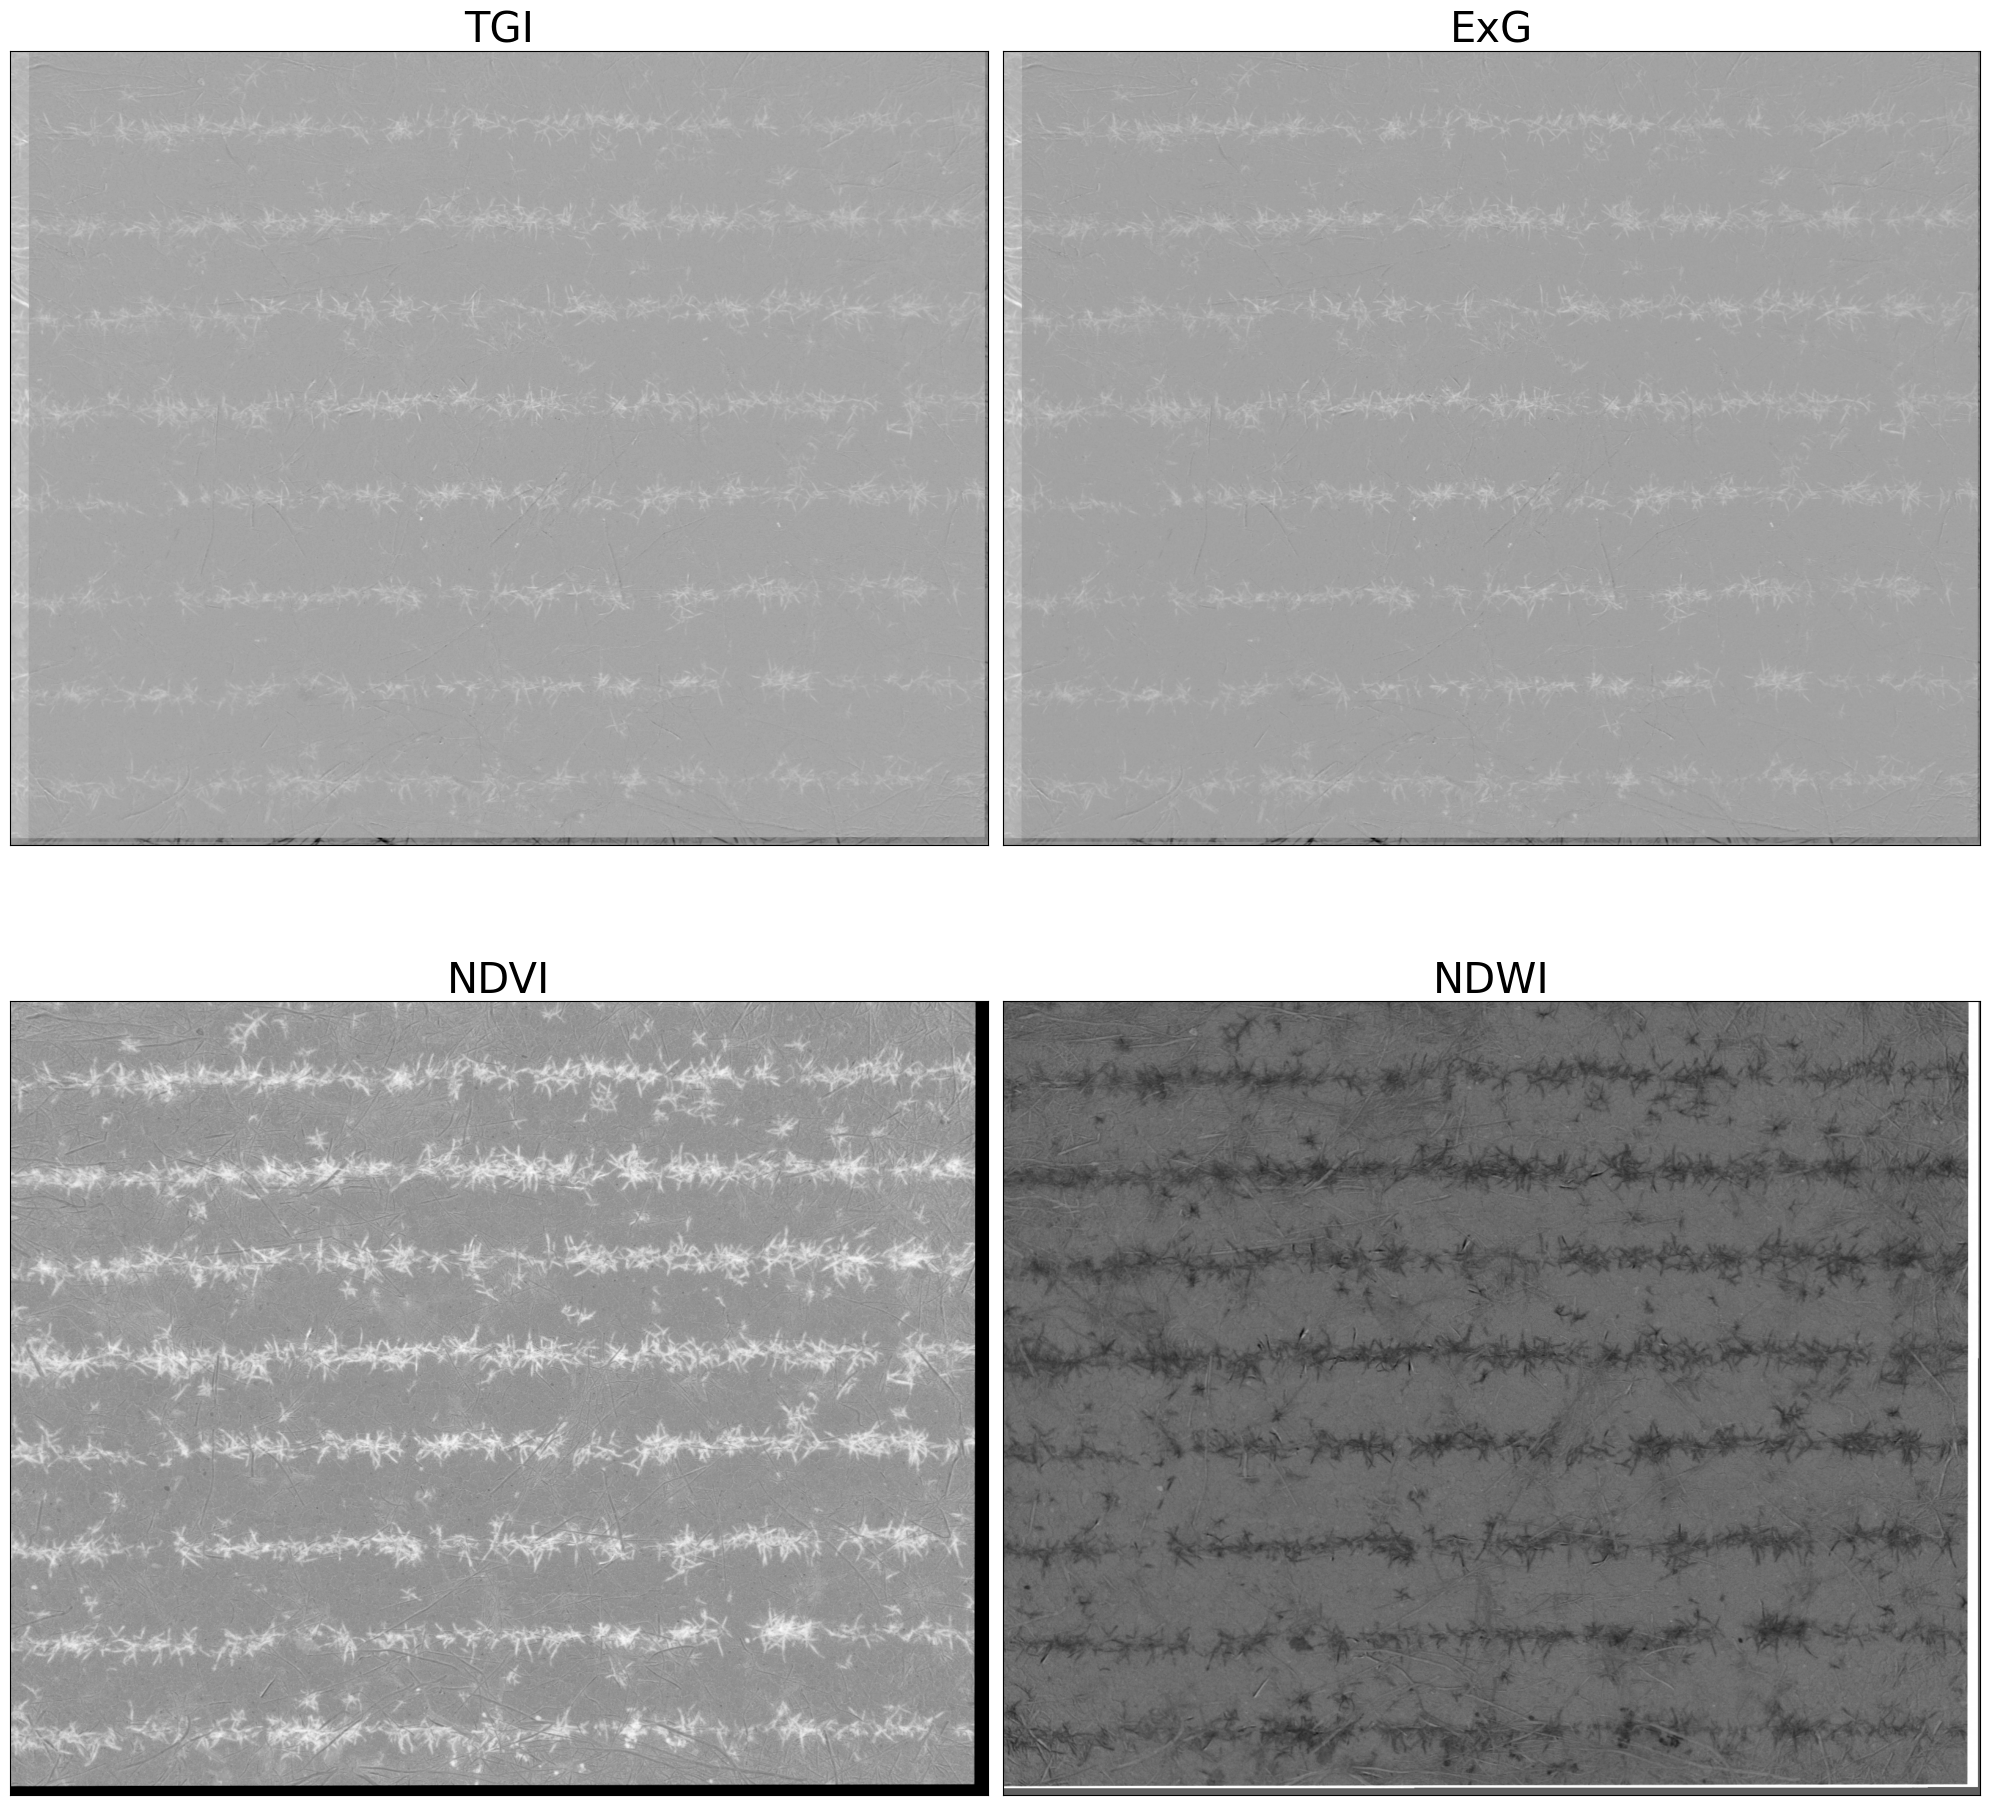
\includegraphics[width=0.95\textwidth]{images/VI_images_no_colorbar.png}
\DIFaddendFL \caption{\DIFdelbeginFL \DIFdelFL{Visualization }\DIFdelendFL \DIFaddbeginFL \DIFaddFL{Qualitative visualization }\DIFaddendFL of the \DIFdelbeginFL \DIFdelFL{vegetation indices }\DIFdelendFL \DIFaddbeginFL \DIFaddFL{vegetation-index images }\DIFaddendFL used in the study. The \DIFdelbeginFL \DIFdelFL{images }\DIFdelendFL \DIFaddbeginFL \DIFaddFL{four panels }\DIFaddendFL show the \DIFaddbeginFL \DIFaddFL{same aligned field scene transformed into }\DIFaddendFL TGI, ExG, NDVI, and NDWI \DIFdelbeginFL \DIFdelFL{images}\DIFdelendFL \DIFaddbeginFL \DIFaddFL{views}\DIFaddendFL . \DIFdelbeginFL \DIFdelFL{The NDVI image highlights the vegetation in the field}\DIFdelendFL \DIFaddbeginFL \DIFaddFL{Each panel is normalized for display}\DIFaddendFL , \DIFdelbeginFL \DIFdelFL{with higher values indicating healthier vegetation. The TGI image emphasizes }\DIFdelendFL \DIFaddbeginFL \DIFaddFL{so }\DIFaddendFL the \DIFdelbeginFL \DIFdelFL{greenness }\DIFdelendFL \DIFaddbeginFL \DIFaddFL{figure should be interpreted as a visual comparison }\DIFaddendFL of \DIFdelbeginFL \DIFdelFL{the vegetation, with higher values indicating more green vegetation. The ExG image enhances the greenness }\DIFdelendFL \DIFaddbeginFL \DIFaddFL{spatial patterns rather than as an axis-based or quantitatively scaled measurement }\DIFaddendFL of \DIFdelbeginFL \DIFdelFL{the vegetation, with higher }\DIFdelendFL \DIFaddbeginFL \DIFaddFL{vegetation-index }\DIFaddendFL values\DIFdelbeginFL \DIFdelFL{indicating greener vegetation}\DIFdelendFL .\DIFdelbeginFL \DIFdelFL{The NDWI image highlights the presence of water in the field, with higher values indicating more water content.}\DIFdelendFL }
    \label{fig:VI-Images}
\end{figure*}

\DIFdelbegin \DIFdel{There is an inverse relationship between the vegetation indices TGI, NDVI, ExG, and the vegetation index NDWI, as illustrated in Figure\ref{fig:VI-Images}. This occurs because }\DIFdelend \DIFaddbegin \DIFadd{Figure~\ref{fig:VI-Images} illustrates that }\DIFaddend TGI, NDVI, and ExG \DIFdelbegin \DIFdel{are optimized to highlight green vegetation : }\DIFdelend \DIFaddbegin \DIFadd{emphasize green vegetation differently from NDWI in this scene. }\DIFaddend TGI and ExG emphasize \DIFdelbegin \DIFdel{green reflectance}\DIFdelend \DIFaddbegin \DIFadd{visible greenness}\DIFaddend , while NDVI \DIFdelbegin \DIFdel{leverages the strong NIR reflectance of chlorophyll in plants, leading to high values in vegetated areas. In contrast, NDWI , designed to identify water bodies by contrasting }\DIFdelend \DIFaddbegin \DIFadd{uses the contrast between NIR and red reflectance. NDWI was originally designed around }\DIFaddend green and NIR reflectance \DIFdelbegin \DIFdel{, shows low values in these vegetated areas due to their high NIR reflectance. Conversely, water bodies, which reflect more green light and less NIR light, exhibit high NDWI values, thereby resulting in the observed inverse relationship}\DIFdelend \DIFaddbegin \DIFadd{and therefore behaves differently for vegetation-dominated pixels. In this study, the figure is used to show qualitative differences among candidate input channels, not to compare absolute VI magnitudes across panels}\DIFaddend .

\subsection{Model \DIFaddbegin \DIFadd{and Training Adaptation}\DIFaddend }

\DIFdelbegin \DIFdel{Our detection model is a modified version of the YOLO }\DIFdelend \DIFaddbegin \DIFadd{The detector is based on a YOLO instance-segmentation }\DIFaddend architecture \cite{Jocher_Ultralytics_YOLO_2023}, adapted to accept multispectral inputs.\DIFaddbegin \footnote{\DIFadd{The reported experiments were implemented with Ultralytics YOLOv8-seg. The article refers to the detector more generally as YOLO-based because the contribution is the multispectral input adaptation and VI-channel comparison rather than a version-specific change to the model family.}} \DIFaddend In contrast to conventional YOLO networks that use RGB images, \DIFdelbegin \DIFdel{our baseline model }\DIFdelend \DIFaddbegin \DIFadd{the baseline configuration }\DIFaddend uses the five aligned spectral bands captured by the UAV (Blue, Green, Red, Red Edge, and Near-Infrared (NIR); see Section~\ref{seq:VI}). \DIFaddbegin \DIFadd{The architecture-level adaptation is the input-channel configuration: the baseline uses five input channels, while the VI configurations use six input channels. The backbone and segmentation head follow the standard YOLO segmentation design; no new detection block is introduced.
}\DIFaddend 

As previous studies have also confirmed, multispectral data can improve detection in agricultural settings by providing spectral information beyond the visible range \DIFdelbegin \DIFdel{\mbox{%DIFAUXCMD
\cite{liu_automated_2023, sportelli_evaluation_2023, dutta_multispectral_2021}}\hskip0pt%DIFAUXCMD
}\DIFdelend \DIFaddbegin \DIFadd{\mbox{%DIFAUXCMD
\cite{liu_automated_2023, sportelli_evaluation_2023, dutta_multispectral_2021, tang_cgs_yolo_2025}}\hskip0pt%DIFAUXCMD
}\DIFaddend . We therefore evaluate whether adding a single vegetation-index (VI) channel to the five-band baseline improves black-grass detection.

The investigated \DIFdelbegin \DIFdel{models }\DIFdelend \DIFaddbegin \DIFadd{input-channel configurations }\DIFaddend are compared to a baseline \emph{5-channel} \DIFdelbegin \DIFdel{model }\DIFdelend \DIFaddbegin \DIFadd{configuration }\DIFaddend (five spectral bands only) and to otherwise identical \DIFdelbegin \DIFdel{models }\DIFdelend \DIFaddbegin \DIFadd{6-channel configurations }\DIFaddend where the same five bands are supplemented with one additional VI channel (NDVI, TGI, ExG, or NDWI). This \DIFdelbegin \DIFdel{is in order to analyze }\DIFdelend \DIFaddbegin \DIFadd{controlled design analyzes }\DIFaddend the impact of each vegetation index separately \DIFaddbegin \DIFadd{while avoiding a comparison across different detector families}\DIFaddend .

\DIFaddbegin \DIFadd{The training loop was adapted to use stacked multispectral arrays rather than RGB images. Because hue-, saturation-, and value-based color augmentation assumes RGB-like image semantics and is not directly meaningful for stacked spectral bands and VI channels, the HSV augmentation terms were disabled in the multispectral training runs. Geometric augmentations and other training settings were handled within the YOLO training framework.
}

\DIFaddend Precise band-to-band alignment is crucial for both vegetation-index computation and reliable training and inference. Accordingly, all spectral bands were geometrically aligned before stacking the channels and feeding them to the network (Figure~\ref{fig:Model-graph}).

\begin{figure*}[t]
    \centering
    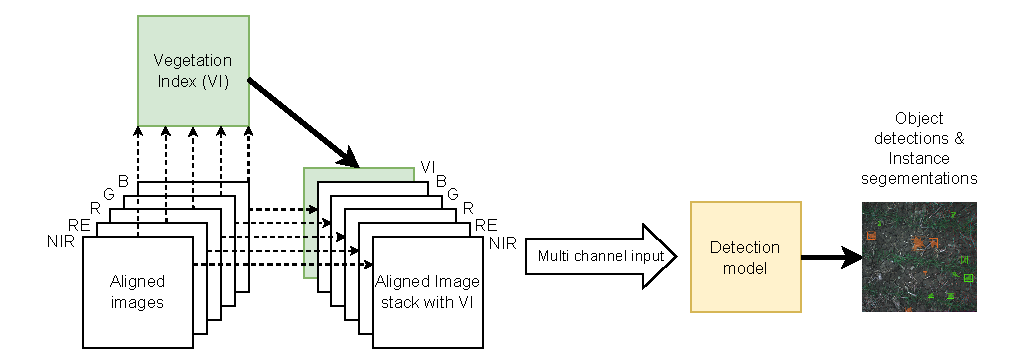
\includegraphics[width=0.95\textwidth]{images/Model Black-grass yolo v2.drawio.pdf}
    \caption{Data-processing pipeline for detecting black-grass. Five aligned multispectral bands (Section~\ref{seq:VI}) are stacked together with an optional vegetation-index channel to form the \DIFdelbeginFL \DIFdelFL{model }\DIFdelendFL \DIFaddbeginFL \DIFaddFL{YOLO segmentation }\DIFaddendFL input used for both training and inference. The baseline (5-channel) \DIFdelbeginFL \DIFdelFL{model }\DIFdelendFL \DIFaddbeginFL \DIFaddFL{configuration }\DIFaddendFL uses only the aligned bands as input\DIFaddbeginFL \DIFaddFL{, while each 6-channel configuration adds one vegetation-index channel}\DIFaddendFL .}
    \label{fig:Model-graph}
\end{figure*}

\DIFaddbegin \begin{table}[t]
\centering
\caption{\DIFaddFL{Reproducibility details for the controlled detector comparison.}}
\label{tab:reproducibility_details}
\scriptsize
\begin{tabular}{p{0.29\linewidth} p{0.55\linewidth}}
\toprule
\textbf{\DIFaddFL{Item}} & \textbf{\DIFaddFL{Description}} \\
\midrule
\DIFaddFL{Detector family }& \DIFaddFL{YOLO instance segmentation with the standard YOLO segmentation backbone and head. }\\
\DIFaddFL{Implementation }& \DIFaddFL{Ultralytics YOLO training with CUDA acceleration configured in the training script; see the method footnote for the implementation version. }\\
\DIFaddFL{Input configurations }& \DIFaddFL{5-channel baseline (B, G, R, RE, NIR) and 6-channel VI configurations (B, G, R, RE, NIR plus one of TGI, ExG, NDVI, or NDWI). }\\
\DIFaddFL{Training data unit }& \DIFaddFL{One aligned UAV image stack from a single drone capture position and its corresponding YOLO segmentation annotation file. The reported detector study did not use a field-scale orthomosaic that was later tiled into smaller detector samples. }\\
\DIFaddFL{Acquisition sessions used in the reported study }& \DIFaddFL{All reported training, validation, and test data in this article were restricted to selected acquisition sessions within the observability window. }\\
\DIFaddFL{Data split }& \DIFaddFL{Train, validation, and test samples were assigned from different field zones. Within the final dataset preparation, annotated image/label files were split into 70\% training, 15\% validation, and 15\% test data. }\\
\DIFaddFL{Multispectral training adaptation }& \DIFaddFL{The training pipeline used stacked multispectral arrays instead of RGB images. RGB-specific HSV augmentation terms were disabled for the multispectral runs. }\\
\DIFaddFL{Evaluation thresholds }& \DIFaddFL{The PR and F1-confidence curves sweep the detector confidence score rather than reporting one fixed operating threshold. AP is computed from the resulting PR behavior after matching predicted and annotated instances. }\\
\DIFaddFL{Bootstrap confidence intervals }& \DIFaddFL{Table~\ref{tab:performance_metrics_by_position} reports 95\% CIs from a detection-level nonparametric bootstrap. Matched detection outcomes and detector confidence scores were resampled with replacement 10}{\DIFaddFL{,}}\DIFaddFL{000 times; AP was recomputed for each resample and CIs are percentile intervals. }\\
\bottomrule
\end{tabular}
\end{table}

\DIFaddend \section{Experiment}

\subsection{Data Acquisition}
The \DIFdelbegin \DIFdel{data was collected from }\DIFdelend \DIFaddbegin \DIFadd{broader acquisition campaign covered }\DIFaddend two winter wheat fields in the south of Sweden. In each field, we had a designated parcel of approximately 20~m $\times$ 20~m. The parcels had a recorded occurrence of black-grass. \DIFaddbegin \DIFadd{The campaign imagery was reviewed across the growing season to identify the period where black-grass could be annotated reliably and where detection would be agronomically useful.
}\DIFaddend 

\DIFaddbegin \DIFadd{We distinguish between two related but separate timing concepts. In this study, the }\emph{\DIFadd{observability window}} \DIFadd{denotes the approximately two- to three-week spring period in which black-grass in the examined winter-wheat fields was sufficiently developed to be visually or spectrally distinguished from wheat, but before wheat growth caused strong occlusion. The }\emph{\DIFadd{susceptibility window}} \DIFadd{denotes the partly overlapping period in which chemical control of black-grass remains biologically and operationally relevant. These windows should be understood as phenological and field-condition-dependent rather than fixed calendar periods: in milder or colder seasons, the same practical window may shift earlier or later depending on local weather, crop development, and weed growth stage. The distinction is important because herbicide efficacy for black-grass is growth-stage dependent; for example, Pintar et al. reported substantially reduced pinoxaden efficacy when applications were delayed to later growth stages \mbox{%DIFAUXCMD
\cite{pintar_growth_stage_2021}}\hskip0pt%DIFAUXCMD
. In Swedish winter-wheat practice, local recommendations likewise frame selective treatment as stage limited rather than universally available throughout the season \mbox{%DIFAUXCMD
\cite{renkavle}}\hskip0pt%DIFAUXCMD
.
}

\DIFaddend The data was collected using a multispectral drone, equipped with five single-band cameras with 2-megapixel (2~MP) sensors: Blue (B), Green (G), Red (R), Red Edge (RE), and Near-Infrared (NIR). The drone was flown at a speed of 1~m/s and altitudes of 1-2~meters, capturing images with a resolution of 0.6-1.2~mm/pixel and consequently an area of 0.8~m $\times$ 1.0~m to 1.6~m $\times$ 2.0~m. 

The \DIFdelbegin \DIFdel{images were captured at different stages of the }\DIFdelend \DIFaddbegin \DIFadd{detector dataset used in the reported experiments was restricted to the selected acquisition sessions on 27~March~2023 and 12~April~2023 across the study fields. No data from earlier or later flights were included in the reported training, validation, or test splits. These two sessions were selected because they fell within the practical overlap between the observability window and the susceptibility window in the studied fields: the wheat had not yet grown over the }\DIFaddend black-grass \DIFdelbegin \DIFdel{growth cycle during the spring, from late February to early June}\DIFdelend \DIFaddbegin \DIFadd{plants, while the black-grass had developed enough to be visually and spectrally differentiated from wheat during annotation. Earlier flights were less useful because the target plants were harder to distinguish, while later flights suffered from increasing crop occlusion and were less aligned with the intended early-season control context}\DIFaddend .

The topography of the parcels featured stiff clay soil interspersed with debris from the previous year's harvest, \DIFdelbegin \DIFdel{presenting challenges such as high reflectance from dead plant material}\DIFdelend \DIFaddbegin \DIFadd{producing bright residue and background structures that complicated visual interpretation in both RGB and VI views}\DIFaddend , see Figures~\ref{fig:VI-Images} and \ref{fig:comparison}. Wheat was sown \DIFdelbegin \DIFdel{in-rows }\DIFdelend \DIFaddbegin \DIFadd{in rows }\DIFaddend spaced 25~cm apart, and images were oriented to capture these rows horizontally, thus maintaining consistency in the viewing angle and direction across all datasets.

\subsection{Annotation}
The data annotation process was critical for preparing the images for training and evaluating the \DIFdelbegin \DIFdel{neural network model }\DIFdelend \DIFaddbegin \DIFadd{detector }\DIFaddend for weed detection. The annotations were conducted using both RGB and NDVI images as references, with human experts carefully reviewing the images to identify and mark the positions of black-grass.

A single experienced annotator performed all annotations, ensuring consistency across the dataset. This annotator was well-versed in recognizing the specific visual characteristics of black-grass and wheat, which can be particularly challenging during their early growth stages when they appear visually similar. To address this challenge, the annotator used NDVI images alongside RGB images. The NDVI images provided additional spectral information that highlighted differences in vegetation health, aiding in the accurate identification of black-grass.

The \DIFaddbegin \DIFadd{NDVI images were used as a visual support source during annotation, not as an automatic labeling rule. Because NDVI was also evaluated as one of the model input channels, this annotation support is an important validity consideration: NDVI-assisted annotation may influence interpretation of the NDVI-channel results. We therefore interpret the NDVI configuration cautiously and focus the main conclusions on the comparative behavior across all VI configurations rather than treating NDVI as a fully independent annotation-free signal.
}

\DIFadd{The }\DIFaddend resulting annotated data included labels specifying the presence of black-grass and its positional relationship to the wheat rows (either within the rows or between the rows).

\subsection{Image Alignment}
As mentioned earlier, the alignment of multispectral images is critical for ensuring that different spectral bands are precisely overlaid for subsequent analysis \cite{pettorelli2013}. The process was done for all the images in the dataset. The alignment also facilitated the computation of the VIs. 

The first step in this process is sensor calibration to remove radial and tangential distortions from multispectral images. Radial distortion results from the lens's shape, whereas tangential distortion is due to imperfection in the lens assembly for each multispectral camera \cite{bradski2008learning}. To correct these distortions, a set of coefficients was computed and applied to the original image coordinates.

After calibration, keypoints are detected and matched across images using the Scale-Invariant Feature Transform (SIFT) \cite{lowe2004}. SIFT detects keypoints and computes descriptors that are invariant to image scaling, translation, rotation, and partially invariant to changes in illumination and affine or 3D projection. Keypoints between images are matched using the nearest neighbor approach in the feature space, followed by a ratio test to refine the matches \cite{muja2009}.

The matched keypoints are then used to compute a transformation matrix that best aligns the two images. This matrix is calculated using a method that minimizes the back-projection error, ensuring that the transformed points in one image match as closely as possible to their corresponding points in the other image \cite{hartley2003}. This process ensures that multispectral images are overlaid precisely, which is fundamental for computing vegetation indices \cite{hallosta_multispectral_2024}. For example, the NDVI is computed using the NIR and red images through this process.

\DIFaddbegin \subsection{\DIFadd{Dataset Construction and Split}}
\DIFadd{The final detector dataset was constructed from aligned multispectral image stacks and their corresponding segmentation annotations. Each training or evaluation sample corresponds to one drone capture position represented by one aligned UAV image stack built from the five spectral bands. The reported detector study did not first generate a field-scale orthomosaic and then tile it into detector patches; instead, the aligned image stacks themselves formed the candidate sample units. No additional overlapping patch-generation step was applied after this stack-generation stage for the reported experiments.
}

\DIFadd{Only image stacks from the selected observability-window sessions that could be annotated reliably were retained for the detector comparison. No image stacks from earlier or later flights were included in the reported detector dataset. The final split was designed so that training, validation, and test samples came from different parts of the field. Within this dataset preparation, the annotated image/label files were split into 70\% training, 15\% validation, and 15\% test data.
}

\DIFadd{This split reduces direct reuse of the same image content across training and evaluation, but it does not remove all possible leakage-like effects. The subsets still come from the same field, acquisition setup, soil background, and narrow crop-growth window. The results should therefore be interpreted as a controlled within-field evaluation of VI-channel effects, not as proof of full geographic or seasonal generalization.
}

\DIFaddend \section{Results}
Our analysis investigates how different vegetation indices influence the network's ability to detect black-grass.
The primary indices considered were the Triangular Greenness Index (TGI), Excess Green Index (ExG), Normalized Difference Vegetation Index (NDVI), and Normalized Difference Water Index (NDWI). These indices were assessed using performance metrics, including average precision (AP), recall, and F1-score. In line with previous studies \cite{su_spectral_2022}, the TGI index shows strong performance on several metrics, indicating that it can enhance detection performance for some operating points.

\DIFaddbegin \DIFadd{In the PR and F1-confidence analyses, the threshold refers to the confidence score assigned by the detector to each predicted instance. The curves therefore show how precision, recall, and F1-score change as this confidence threshold is swept, rather than reporting performance at a single fixed threshold.
}

\DIFaddend \begin{figure*}[htbp]
    \centering
    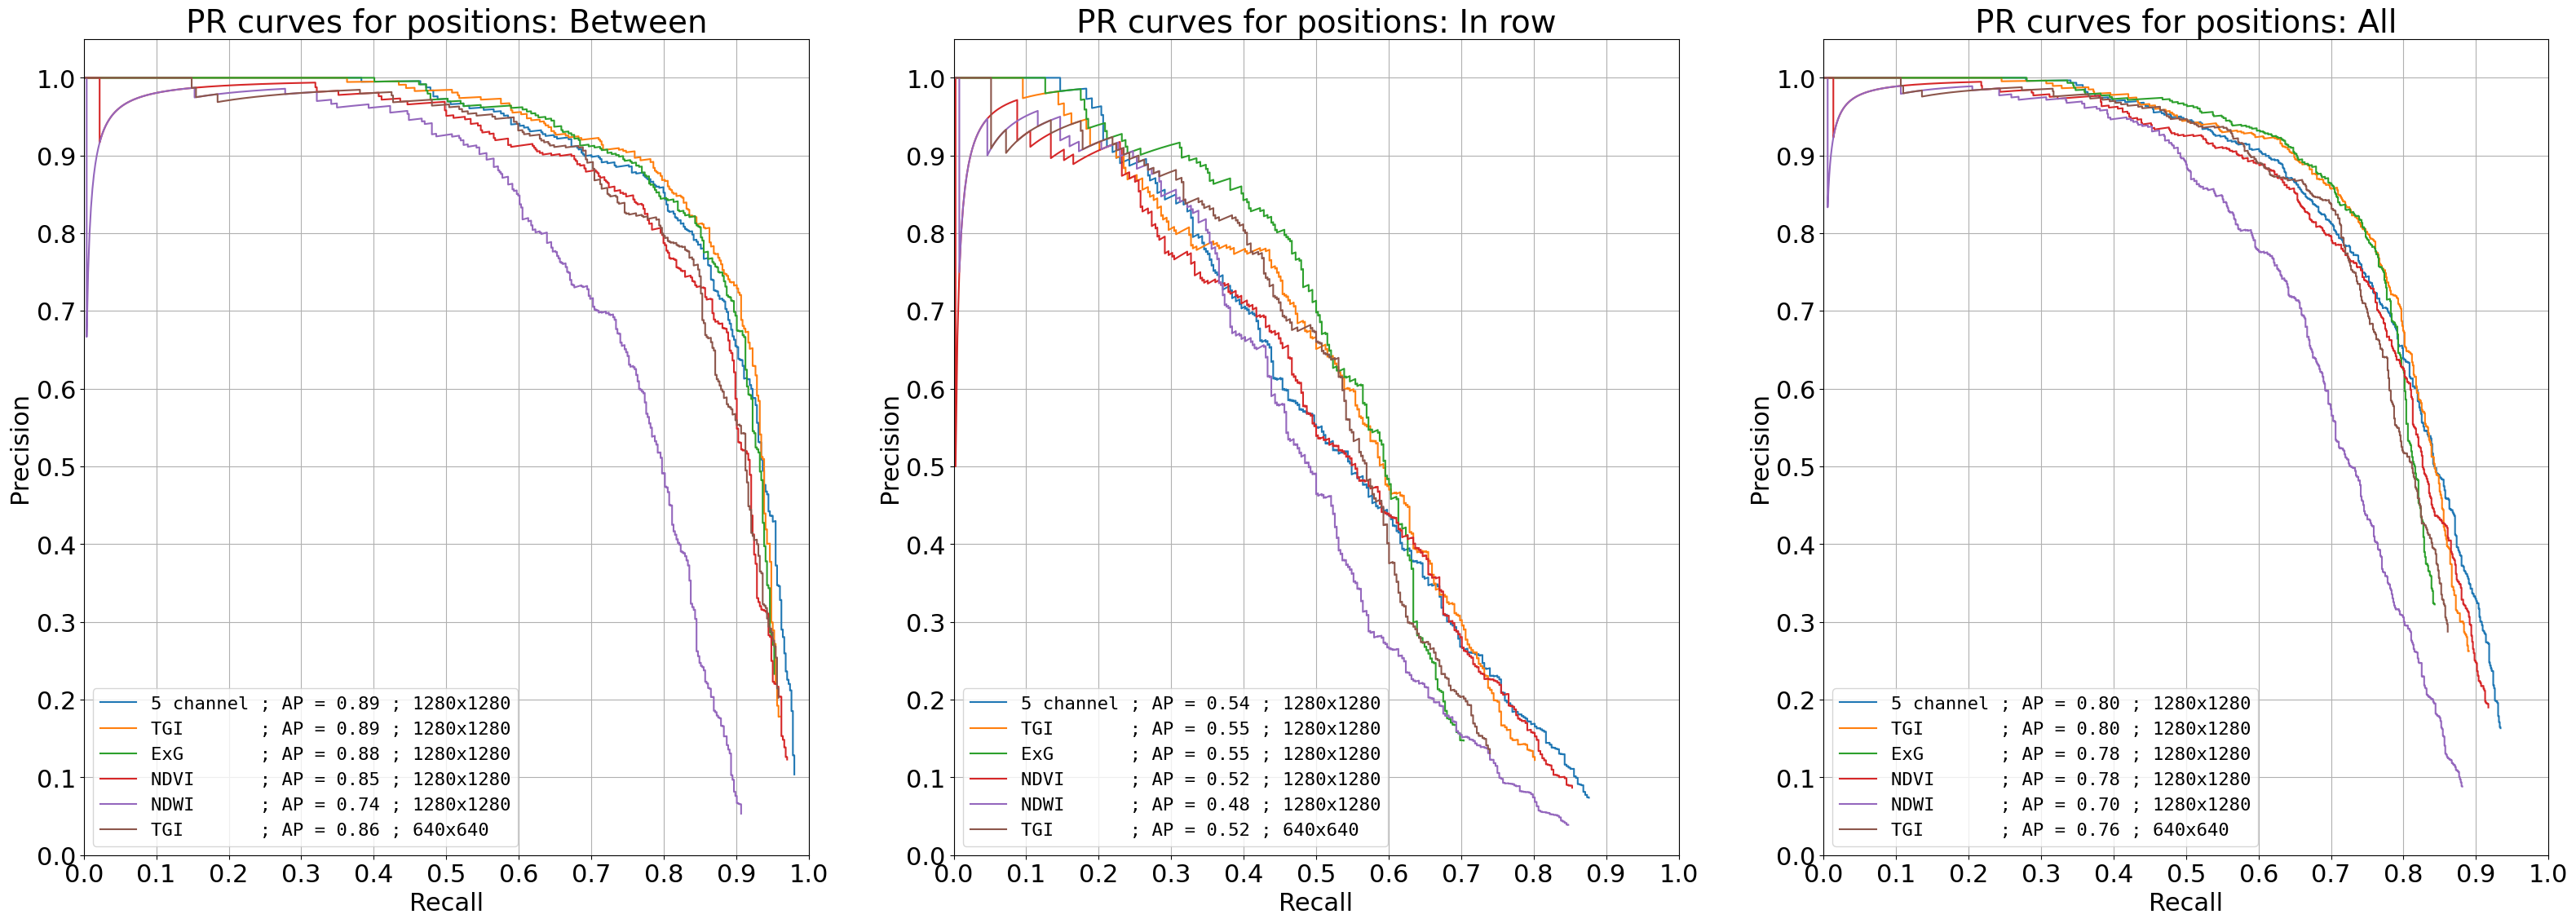
\includegraphics[width=1\textwidth]{images/PR-curves_Different_Positions_v3.png}
    \caption{\DIFdelbeginFL \DIFdelFL{Precision-Recall }\DIFdelendFL \DIFaddbeginFL \DIFaddFL{Precision--recall }\DIFaddendFL (PR) curves for different \DIFdelbeginFL \DIFdelFL{models }\DIFdelendFL \DIFaddbeginFL \DIFaddFL{input-channel configurations }\DIFaddendFL across three positional categories: Between, In row, and All. The \DIFdelbeginFL \DIFdelFL{models }\DIFdelendFL \DIFaddbeginFL \DIFaddFL{configurations }\DIFaddendFL evaluated are the 5-channel \DIFdelbeginFL \DIFdelFL{model, }\DIFdelendFL \DIFaddbeginFL \DIFaddFL{baseline and the }\DIFaddendFL TGI, ExG, NDVI, \DIFaddbeginFL \DIFaddFL{and }\DIFaddendFL NDWI \DIFaddbeginFL \DIFaddFL{configurations }\DIFaddendFL at \DIFdelbeginFL \DIFdelFL{a }\DIFdelendFL \DIFaddbeginFL \DIFaddFL{1280$\times$1280 }\DIFaddendFL resolution\DIFdelbeginFL \DIFdelFL{of 1280x1280}\DIFdelendFL , \DIFdelbeginFL \DIFdelFL{and }\DIFdelendFL \DIFaddbeginFL \DIFaddFL{plus one additional }\DIFaddendFL TGI \DIFaddbeginFL \DIFaddFL{probe }\DIFaddendFL at \DIFdelbeginFL \DIFdelFL{a resolution of 640x640. }\DIFdelendFL \DIFaddbeginFL \DIFaddFL{640$\times$640. }\DIFaddendFL The PR curves illustrate the trade-off between precision and recall \DIFdelbeginFL \DIFdelFL{for each model, with the Average Precision (AP) indicating overall performance}\DIFdelendFL \DIFaddbeginFL \DIFaddFL{as detector confidence scores are swept}\DIFaddendFL .}
    \label{fig:PR-curves-positions}
\end{figure*}

\subsection{Precision--recall characteristics across confidence thresholds}
As illustrated in Figure~\ref{fig:PR-curves-positions}, the precision--recall (PR) curves \DIFdelbegin \DIFdel{demonstrate that models utilizing }\DIFdelend \DIFaddbegin \DIFadd{show that }\DIFaddend the Triangular Greenness Index (TGI) and Excess Green Index (ExG) \DIFaddbegin \DIFadd{configurations }\DIFaddend maintain higher precision \DIFdelbegin \DIFdel{while achieving substantial recall values across different positional categories. This robustness underscores their effectiveness in distinguishing }\DIFdelend \DIFaddbegin \DIFadd{over substantial parts of the recall range in the evaluated field data. This suggests that these VI channels can help distinguish }\DIFaddend black-grass from wheat under \DIFdelbegin \DIFdel{varied conditions. Specifically, the TGI model consistently outperforms other models in both ``between rows'' and ``}\DIFdelend \DIFaddbegin \DIFadd{the reported acquisition conditions. The effect is clearest between rows, while all configurations remain more challenged }\DIFaddend in-row \DIFdelbegin \DIFdel{'' positions, indicating that it generalizes well across the two spatial contexts. Additionally, it is noteworthy that while the }\DIFdelend \DIFaddbegin \DIFadd{because wheat occlusion and weed--crop similarity are higher. The }\DIFaddend baseline 5-channel \DIFdelbegin \DIFdel{model achieves high recall , it suffers from lower precision at the beginning of the PR curves}\DIFdelend \DIFaddbegin \DIFadd{configuration reaches high recall at lower confidence thresholds, but with lower precision in parts of the sweep}\DIFaddend . This trade-off is further emphasized in the F1-score curves shown in Figure~\ref{fig:F1-curves-positions}\DIFdelbegin \DIFdel{, where the baseline model exhibits a lower overall F1-score across confidence thresholds compared to most models incorporating an additional vegetation index channel}\DIFdelend .

\subsection{Average Precision (AP) and confidence intervals (CIs)}
To provide a threshold-aggregated summary of detection performance, we report Average Precision (AP) \cite{lin_coco_2014} together with 95\% confidence intervals (CIs) \DIFaddbegin \DIFadd{from a detection-level nonparametric bootstrap \mbox{%DIFAUXCMD
\cite{efron1979bootstrap}}\hskip0pt%DIFAUXCMD
.
For each input-channel configuration and positional subset, predictions were first matched to annotated instances using the same matching procedure used for the PR analysis. The matched detection outcomes and detector confidence scores were resampled with replacement 10}{\DIFadd{,}}\DIFadd{000 times. For each bootstrap resample, the PR curve and AP were recomputed, and the 95\% CI was defined by the 2.5th and 97.5th percentiles of the resulting AP distribution}\DIFaddend .
\DIFdelbegin \DIFdel{Confidence intervals were computed using bootstrap resampling \mbox{%DIFAUXCMD
\cite{efron1979bootstrap}}\hskip0pt%DIFAUXCMD
.
}\DIFdelend For completeness, we also report results for a TGI \DIFdelbegin \DIFdel{model }\DIFdelend \DIFaddbegin \DIFadd{configuration }\DIFaddend trained at a reduced input resolution (640$\times$640), whereas the remaining \DIFdelbegin \DIFdel{models }\DIFdelend \DIFaddbegin \DIFadd{configurations }\DIFaddend were trained and evaluated at 1280$\times$1280.
Table~\ref{tab:performance_metrics_by_position} presents the AP values and their 95\% confidence intervals for each \DIFdelbegin \DIFdel{model }\DIFdelend \DIFaddbegin \DIFadd{configuration }\DIFaddend and positional category. Key observations include:
\begin{itemize}
    \item \textbf{Between Rows:} The TGI \DIFdelbegin \DIFdel{model }\DIFdelend \DIFaddbegin \DIFadd{configuration }\DIFaddend achieves the highest AP (0.892), closely followed by the 5-channel \DIFdelbegin \DIFdel{model }\DIFdelend \DIFaddbegin \DIFadd{baseline }\DIFaddend (0.889). The NDWI \DIFdelbegin \DIFdel{model }\DIFdelend \DIFaddbegin \DIFadd{configuration }\DIFaddend underperforms with an AP of 0.742.
    \item \textbf{In Rows:} All \DIFdelbegin \DIFdel{models }\DIFdelend \DIFaddbegin \DIFadd{configurations }\DIFaddend show reduced performance due to occlusion by wheat. The TGI \DIFdelbegin \DIFdel{model }\DIFdelend \DIFaddbegin \DIFadd{configuration }\DIFaddend maintains a relatively higher performance (AP~=~0.553), closely followed by ExG (AP~=~0.547), \mbox{5-channel (AP~=~0.545)} and NDVI (AP~=~0.523).
    \item \textbf{All:} The 5-channel \DIFdelbegin \DIFdel{model }\DIFdelend \DIFaddbegin \DIFadd{baseline }\DIFaddend achieves the highest AP of 0.805, followed by the TGI \DIFdelbegin \DIFdel{model }\DIFdelend \DIFaddbegin \DIFadd{configuration }\DIFaddend (1280$\times$1280) with an AP of 0.800. While the baseline is marginally higher on the combined set, the TGI \DIFdelbegin \DIFdel{model }\DIFdelend \DIFaddbegin \DIFadd{configuration }\DIFaddend performs comparatively better when the data are analyzed separately by positional category, suggesting that the overall ranking is influenced by the composition of the combined dataset.
\end{itemize}

\begin{table}[htbp]
\centering
\caption{Average Precision (AP) values for each \DIFdelbeginFL \DIFdelFL{model }\DIFdelendFL \DIFaddbeginFL \DIFaddFL{input-channel configuration }\DIFaddendFL and position, along with their corresponding 95\% confidence intervals \DIFdelbeginFL \DIFdelFL{. Confidence intervals were computed using 10000 }\DIFdelendFL \DIFaddbeginFL \DIFaddFL{from the detection-level 10}{\DIFaddFL{,}}\DIFaddFL{000-resample }\DIFaddendFL bootstrap \DIFdelbeginFL \DIFdelFL{resamples}\DIFdelendFL \DIFaddbeginFL \DIFaddFL{analysis}\DIFaddendFL .}
\begin{tabular}{lll}
\toprule
\multicolumn{1}{c}{\DIFdelbeginFL \textbf{\DIFdelFL{Model}}%DIFAUXCMD
\DIFdelendFL \DIFaddbeginFL \textbf{\DIFaddFL{Configuration}}\DIFaddendFL } & \multicolumn{1}{c}{\textbf{AP}} & \multicolumn{1}{c}{\textbf{95\% CI}} \\
\midrule
\multicolumn{3}{c}{\textbf{Position: Between}} \\
\DIFdelbeginFL \DIFdelFL{5 channel 1280x1280 }\DIFdelendFL \DIFaddbeginFL \DIFaddFL{5-channel 1280$\times$1280 }\DIFaddendFL & 0.889 & (0.810 - 0.971) \\
\textbf{TGI \DIFdelbeginFL \DIFdelFL{1280x1280}\DIFdelendFL \DIFaddbeginFL \DIFaddFL{1280$\times$1280}\DIFaddendFL } & \textbf{0.892} & \textbf{(0.812 - 0.970)} \\
ExG \DIFdelbeginFL \DIFdelFL{1280x1280 }\DIFdelendFL \DIFaddbeginFL \DIFaddFL{1280$\times$1280 }\DIFaddendFL & 0.884 & (0.808 - 0.959) \\
NDVI \DIFdelbeginFL \DIFdelFL{1280x1280 }\DIFdelendFL \DIFaddbeginFL \DIFaddFL{1280$\times$1280 }\DIFaddendFL & 0.855 & (0.773 - 0.935) \\
NDWI \DIFdelbeginFL \DIFdelFL{1280x1280 }\DIFdelendFL \DIFaddbeginFL \DIFaddFL{1280$\times$1280 }\DIFaddendFL & 0.742 & (0.660 - 0.823) \\
TGI \DIFdelbeginFL \DIFdelFL{640x640 }\DIFdelendFL \DIFaddbeginFL \DIFaddFL{640$\times$640 }\DIFaddendFL & 0.856 & (0.776 - 0.933) \\
\midrule
\multicolumn{3}{c}{\textbf{Position: In rows}} \\
\DIFdelbeginFL \DIFdelFL{5 channel 1280x1280 }\DIFdelendFL \DIFaddbeginFL \DIFaddFL{5-channel 1280$\times$1280 }\DIFaddendFL & 0.545 & (0.467 - 0.625) \\
\textbf{TGI \DIFdelbeginFL \DIFdelFL{1280x1280}\DIFdelendFL \DIFaddbeginFL \DIFaddFL{1280$\times$1280}\DIFaddendFL } & \textbf{0.553} & \textbf{(0.473 - 0.635)} \\
ExG \DIFdelbeginFL \DIFdelFL{1280x1280 }\DIFdelendFL \DIFaddbeginFL \DIFaddFL{1280$\times$1280 }\DIFaddendFL & 0.547 & (0.472 - 0.625) \\
NDVI \DIFdelbeginFL \DIFdelFL{1280x1280 }\DIFdelendFL \DIFaddbeginFL \DIFaddFL{1280$\times$1280 }\DIFaddendFL & 0.523 & (0.440 - 0.607) \\
NDWI \DIFdelbeginFL \DIFdelFL{1280x1280 }\DIFdelendFL \DIFaddbeginFL \DIFaddFL{1280$\times$1280 }\DIFaddendFL & 0.483 & (0.405 - 0.561) \\
TGI \DIFdelbeginFL \DIFdelFL{640x640 }\DIFdelendFL \DIFaddbeginFL \DIFaddFL{640$\times$640 }\DIFaddendFL & 0.525 & (0.447 - 0.603) \\
\midrule
\multicolumn{3}{c}{\textbf{Position: All}} \\
\textbf{\DIFdelbeginFL \DIFdelFL{5 channel 1280x1280}\DIFdelendFL \DIFaddbeginFL \DIFaddFL{5-channel 1280$\times$1280}\DIFaddendFL } & \textbf{0.805} & \textbf{(0.748 - 0.865)} \\
TGI \DIFdelbeginFL \DIFdelFL{1280x1280 }\DIFdelendFL \DIFaddbeginFL \DIFaddFL{1280$\times$1280 }\DIFaddendFL & 0.800 & (0.746 - 0.854) \\
ExG \DIFdelbeginFL \DIFdelFL{1280x1280 }\DIFdelendFL \DIFaddbeginFL \DIFaddFL{1280$\times$1280 }\DIFaddendFL & 0.778 & (0.728 - 0.829) \\
NDVI \DIFdelbeginFL \DIFdelFL{1280x1280 }\DIFdelendFL \DIFaddbeginFL \DIFaddFL{1280$\times$1280 }\DIFaddendFL & 0.783 & (0.727 - 0.840) \\
NDWI \DIFdelbeginFL \DIFdelFL{1280x1280 }\DIFdelendFL \DIFaddbeginFL \DIFaddFL{1280$\times$1280 }\DIFaddendFL & 0.696 & (0.640 - 0.754) \\
TGI \DIFdelbeginFL \DIFdelFL{640x640 }\DIFdelendFL \DIFaddbeginFL \DIFaddFL{640$\times$640 }\DIFaddendFL & 0.765 & (0.711 - 0.818) \\
\bottomrule
\end{tabular}
\label{tab:performance_metrics_by_position}
\end{table}

\begin{figure*}[htbp]
    \centering
    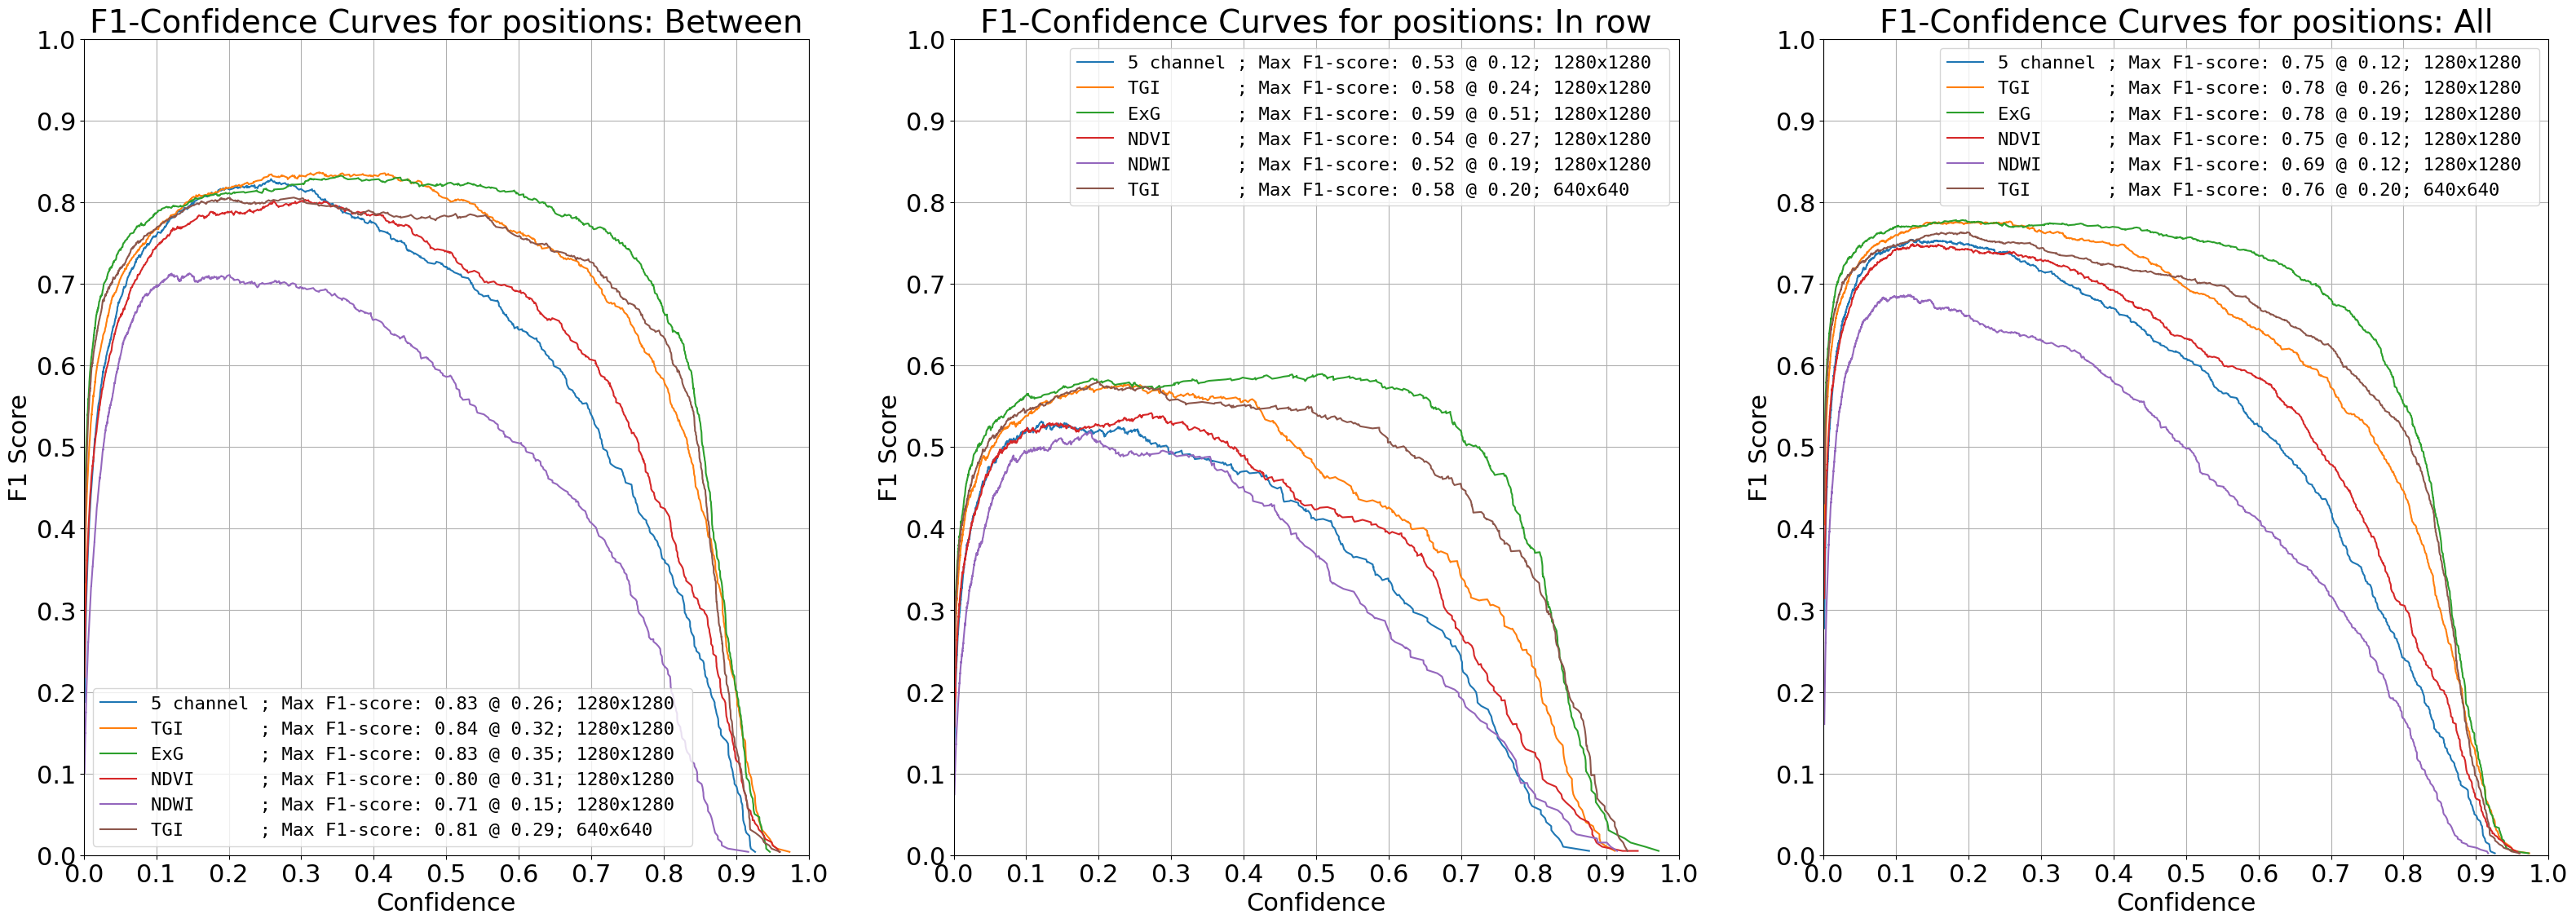
\includegraphics[width=1\textwidth]{images/F1-Confidence-curves_Different_Positions_v3.png}
    \caption{\DIFdelbeginFL \DIFdelFL{F1-Confidence }\DIFdelendFL \DIFaddbeginFL \DIFaddFL{F1-confidence }\DIFaddendFL curves for different \DIFdelbeginFL \DIFdelFL{models }\DIFdelendFL \DIFaddbeginFL \DIFaddFL{input-channel configurations }\DIFaddendFL across three positional categories: Between, In row, and All. The \DIFdelbeginFL \DIFdelFL{models }\DIFdelendFL \DIFaddbeginFL \DIFaddFL{configurations }\DIFaddendFL evaluated include the \DIFdelbeginFL \DIFdelFL{5 channel model, }\DIFdelendFL \DIFaddbeginFL \DIFaddFL{5-channel baseline and the }\DIFaddendFL TGI, ExG, NDVI, \DIFaddbeginFL \DIFaddFL{and }\DIFaddendFL NDWI \DIFaddbeginFL \DIFaddFL{configurations }\DIFaddendFL at \DIFdelbeginFL \DIFdelFL{a }\DIFdelendFL \DIFaddbeginFL \DIFaddFL{1280$\times$1280 }\DIFaddendFL resolution\DIFdelbeginFL \DIFdelFL{of 1280x1280}\DIFdelendFL , \DIFdelbeginFL \DIFdelFL{and }\DIFdelendFL \DIFaddbeginFL \DIFaddFL{plus one additional }\DIFaddendFL TGI \DIFaddbeginFL \DIFaddFL{probe }\DIFaddendFL at \DIFdelbeginFL \DIFdelFL{a resolution of 640x640. }\DIFdelendFL \DIFaddbeginFL \DIFaddFL{640$\times$640. }\DIFaddendFL The F1 score represents the harmonic mean of precision and recall \DIFdelbeginFL \DIFdelFL{, providing a balanced measure of the models' performance }\DIFdelendFL as a function of \DIFaddbeginFL \DIFaddFL{detector }\DIFaddendFL confidence score.}
    \label{fig:F1-curves-positions}
\end{figure*}

Figures~\ref{fig:PR-curves-positions} and \ref{fig:F1-curves-positions} depict PR behavior and F1-confidence curves, respectively. Together, these curves highlight the precision--recall trade-off when selecting confidence thresholds for practical deployment. In particular, the TGI and ExG \DIFdelbegin \DIFdel{models }\DIFdelend \DIFaddbegin \DIFadd{configurations }\DIFaddend tend to achieve more balanced performance across thresholds, whereas the baseline 5-channel \DIFdelbegin \DIFdel{model }\DIFdelend \DIFaddbegin \DIFadd{configuration }\DIFaddend reaches high recall at the cost of lower precision at lower confidence thresholds.

The detailed analysis reveals several key insights:
\begin{itemize}
    \item \textbf{\DIFdelbegin \DIFdel{Model }\DIFdelend \DIFaddbegin \DIFadd{Configuration }\DIFaddend Performance:} The \DIFdelbegin \DIFdel{TGI model trained on }\DIFdelend \DIFaddbegin \DIFadd{additional TGI run at }\DIFaddend lower resolution (\DIFdelbegin \DIFdel{640x640) outperforms the NDWI model, highlighting the significance of the vegetation index relative to image resolution in this comparison}\DIFdelend \DIFaddbegin \DIFadd{640$\times$640) remains competitive with some 1280$\times$1280 configurations, but it should be interpreted only as a targeted probe because equivalent lower-resolution runs were not available for the other VIs}\DIFaddend .
    \item \textbf{Positional Differences:} There is a notable difference in detection performance between weeds located between rows and those within rows, with better performance in less occluded conditions. This underscores the need for robust detection under occlusion.
\end{itemize}

The bootstrap confidence intervals quantify uncertainty in the AP estimates \DIFdelbegin \DIFdel{due to finite test-set sampling \mbox{%DIFAUXCMD
\cite{efron1979bootstrap}}\hskip0pt%DIFAUXCMD
}\DIFdelend \DIFaddbegin \DIFadd{under this matched detection-outcome resampling scheme, not variation across new fields or seasons}\DIFaddend .

\section{Discussion}
Our study investigates the impact of different vegetation indices on the performance of neural networks in detecting black-grass using UAV-acquired multispectral images. The main findings are as follows:

\begin{itemize}
    \item The TGI index demonstrated \DIFdelbegin \DIFdel{enhanced performance}\DIFdelend \DIFaddbegin \DIFadd{the strongest AP in the between-row and in-row categories}\DIFaddend , closely followed by the ExG index\DIFdelbegin \DIFdel{. Both indices outperformed }\DIFdelend \DIFaddbegin \DIFadd{, while }\DIFaddend the 5-channel baseline \DIFdelbegin \DIFdel{model in terms of precision while maintaining high recall values}\DIFdelend \DIFaddbegin \DIFadd{remained strongest in the combined AP summary}\DIFaddend .
    \item The NDWI index underperformed compared to the other indices, negatively impacting the \DIFdelbegin \DIFdel{model’s detection capabilities}\DIFdelend \DIFaddbegin \DIFadd{detector's performance in this configuration}\DIFaddend .
    \item The \DIFdelbegin \DIFdel{choice of vegetation index can mitigate the limitations of lower resolution images, as seen with the TGI model at 640x640 resolution performing better than the NDWI model}\DIFdelend \DIFaddbegin \DIFadd{targeted TGI 640$\times$640 probe remained competitive with some 1280$\times$1280 configurations, but the study does not establish a general resolution trend across all VIs}\DIFaddend .
    \item The \DIFdelbegin \DIFdel{5-channeled baseline model }\DIFdelend \DIFaddbegin \DIFadd{5-channel baseline configuration }\DIFaddend achieved the highest overall recall.
\end{itemize}

\subsection{\DIFdelbegin \DIFdel{Model }\DIFdelend \DIFaddbegin \DIFadd{Configuration }\DIFaddend Performance and Interpretation}
The \DIFdelbegin \DIFdel{increased performance }\DIFdelend \DIFaddbegin \DIFadd{favorable behavior }\DIFaddend of the TGI and ExG \DIFdelbegin \DIFdel{indices can be attributed to their ability to preserve the color }\DIFdelend \DIFaddbegin \DIFadd{configurations is likely related to how these indices preserve visible greenness }\DIFaddend differences between black-grass and wheat \DIFdelbegin \DIFdel{more effectively. These indices' lower contrast and broader value range contribute to better detection outcomes. This finding }\DIFdelend \DIFaddbegin \DIFadd{in the reported scenes. This interpretation }\DIFaddend is consistent with the results of Su et al., who found that specific vegetation indices can improve the accuracy of \DIFdelbegin \DIFdel{weed detection }\DIFdelend \DIFaddbegin \DIFadd{black-grass weed mapping }\DIFaddend models \cite{su_spectral_2022}. \DIFaddbegin \DIFadd{It also aligns with recent black-grass studies showing that multispectral and hyperspectral cues are informative in cereal crops, while also being sensitive to acquisition setting and between-site variation \mbox{%DIFAUXCMD
\cite{cox_black-grass_2023, goodsell_black_grass_2024, darbyshire_blackgrass_2025}}\hskip0pt%DIFAUXCMD
.
}\DIFaddend 

\DIFdelbegin \DIFdel{In contrast, the NDWI index's negative values for vegetative regions might have hindered the model’s learning process, resulting in poorer performance.
This hypothesis is supported by Lambert }\DIFdelend \DIFaddbegin \DIFadd{The comparison with Darbyshire }\DIFaddend et al.\DIFdelbegin \DIFdel{, who noted challenges in model transferability across different environmental conditions, which could be exacerbated by indices that do not align well }\DIFdelend \DIFaddbegin \DIFadd{~\mbox{%DIFAUXCMD
\cite{darbyshire_blackgrass_2025} }\hskip0pt%DIFAUXCMD
is most informative when viewed through the evaluation task rather than the headline score. Their reported 89.6\% image-level classification accuracy and the between-row AP of 0.892 for our TGI configuration are numerically similar, but they measure different errors: classification can succeed by assigning the correct class to an image, whereas instance segmentation requires individual black-grass instances to be localized with sufficient overlap and confidence. The lower in-row AP (0.553 for TGI) therefore suggests that the harder part of the present problem is not only recognizing a black-grass spectral signature, but preserving instance-level localization under wheat occlusion and crop--weed similarity.
}

\DIFadd{In contrast, the NDWI configuration appears less aligned }\DIFaddend with the spectral \DIFdelbegin \DIFdel{properties of the target vegetation }\DIFdelend \DIFaddbegin \DIFadd{cues that separated black-grass from wheat in this dataset. This weaker behavior should be interpreted in the context of site-specific spectral conditions, since previous work has shown that weed-mapping performance can vary with environmental conditions and acquisition setting }\DIFaddend \cite{lambert_evaluating_2018}.

The 5-channel \DIFdelbegin \DIFdel{model }\DIFdelend \DIFaddbegin \DIFadd{baseline configuration }\DIFaddend achieved the highest recall, indicating its effectiveness in detecting most occurrences of black-grass. However, the TGI and ExG \DIFdelbegin \DIFdel{models }\DIFdelend \DIFaddbegin \DIFadd{configurations }\DIFaddend maintained higher precision, providing more reliable detections with fewer false positives. This trade-off is crucial depending on the \DIFdelbegin \DIFdel{application—whether }\DIFdelend \DIFaddbegin \DIFadd{application--whether }\DIFaddend the goal is to detect all weeds or to ensure precise detection with minimal errors.

\subsection{Detection Between and In Rows}
An essential aspect of our findings is the difference in detection performance between rows and within rows of wheat. Figures~\ref{fig:PR-curves-positions} and \ref{fig:F1-curves-positions}, along with Table \ref{tab:performance_metrics_by_position}, show that \DIFdelbegin \DIFdel{models }\DIFdelend \DIFaddbegin \DIFadd{the configurations }\DIFaddend are more successful in identifying black-grass between rows, where there is less occlusion and higher contrast. In-row detection is hindered by occlusion and visual similarity between wheat and black-grass, leading to lower precision and recall. For instance, the TGI \DIFdelbegin \DIFdel{model }\DIFdelend \DIFaddbegin \DIFadd{configuration }\DIFaddend achieved an AP of 0.892 between rows compared to 0.553 within rows. This highlights the need for advanced techniques to improve in-row detection, which remains a significant challenge for UAV-based weed detection.

\begin{figure*}[h]%[htbp]
    \centering
    \subfigure[Original RGB image]{%
        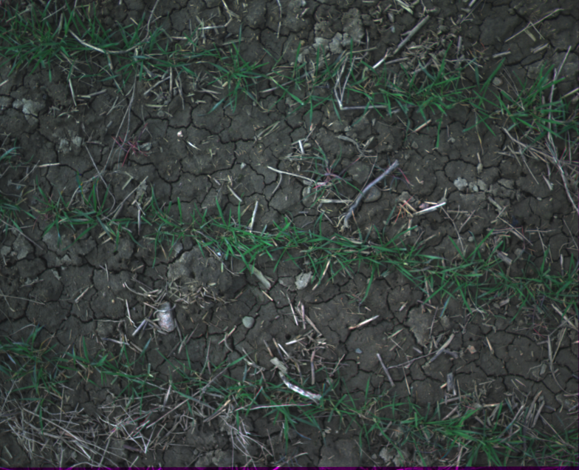
\includegraphics[width=0.3\textwidth]{images/Original-RGB.png}
    }\hfill
    \subfigure[Predictions in RGB image]{%
        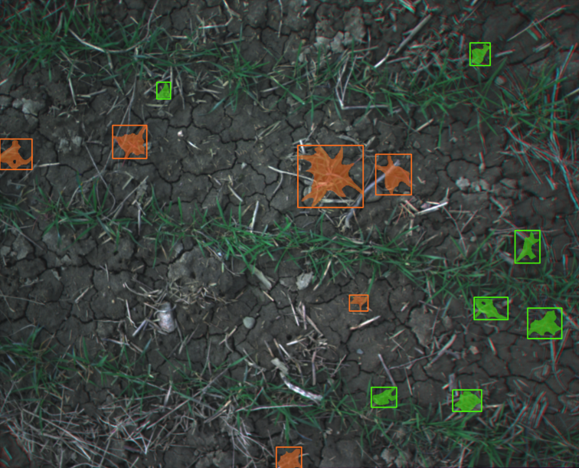
\includegraphics[width=0.3\textwidth]{images/Predictions-rgb.png}
    }\hfill
    \subfigure[Annotations in NDVI image]{%
        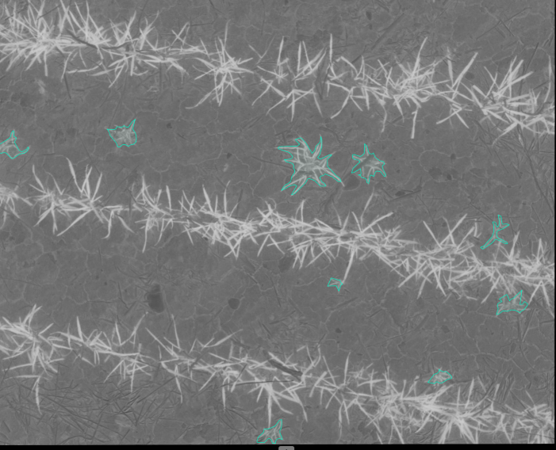
\includegraphics[width=0.3\textwidth]{images/Annotation-NDVI.png}
    }
    \caption{\DIFdelbeginFL \DIFdelFL{Comparison }\DIFdelendFL \DIFaddbeginFL \DIFaddFL{Qualitative comparison }\DIFaddendFL of the original RGB image (a), \DIFdelbeginFL \DIFdelFL{the }\DIFdelendFL \DIFaddbeginFL \DIFaddFL{detector }\DIFaddendFL predictions \DIFaddbeginFL \DIFaddFL{shown }\DIFaddendFL on the RGB image (b), and annotations \DIFaddbeginFL \DIFaddFL{shown }\DIFaddendFL on the NDVI image \DIFaddbeginFL \DIFaddFL{used during labeling }\DIFaddendFL (c). \DIFdelbeginFL \DIFdelFL{The images illustrate the model's ability to detect annotated instances of black-grass while also suggesting highly probable candidates that may have been missed during annotation. The orange }\DIFdelendFL \DIFaddbeginFL \DIFaddFL{Orange }\DIFaddendFL markings indicate black-grass classified as \DIFdelbeginFL \DIFdelFL{"}\DIFdelendFL between \DIFdelbeginFL \DIFdelFL{the }\DIFdelendFL rows, \DIFdelbeginFL \DIFdelFL{" }\DIFdelendFL while \DIFdelbeginFL \DIFdelFL{the }\DIFdelendFL green masks \DIFdelbeginFL \DIFdelFL{show instances considered as }\DIFdelendFL \DIFaddbeginFL \DIFaddFL{indicate black-grass }\DIFaddendFL located \DIFdelbeginFL \DIFdelFL{"}\DIFdelendFL in the wheat rows. \DIFdelbeginFL \DIFdelFL{" }\DIFdelendFL The \DIFdelbeginFL \DIFdelFL{model }\DIFdelendFL \DIFaddbeginFL \DIFaddFL{detector }\DIFaddendFL used for predictions is the reference \DIFdelbeginFL \DIFdelFL{model, }\DIFdelendFL \DIFaddbeginFL \DIFaddFL{5-channel configuration }\DIFaddendFL trained on the original five image bands.}
    \label{fig:comparison}
\end{figure*}

\subsection{\DIFdelbegin \DIFdel{Implications }\DIFdelend \DIFaddbegin \DIFadd{Qualitative Interpretation }\DIFaddend of \DIFdelbegin \DIFdel{Model }\DIFdelend Predictions \DIFdelbegin \DIFdel{Compared to }\DIFdelend \DIFaddbegin \DIFadd{and }\DIFaddend Annotations}

Figure\DIFdelbegin \DIFdel{\ref{fig:comparison} provides visual comparisons of original RGB images, model }\DIFdelend \DIFaddbegin \DIFadd{~\ref{fig:comparison} compares the original RGB view, detector }\DIFaddend predictions, and \DIFdelbegin \DIFdel{NDVI annotations, showcasing the network's proficiency in detecting black-grass amidst wheat. The model identifies highly probable candidates for black-grass, some of which may actually be instances of black-grass that were missed during the annotation stage. This observation suggests that certain false positives impacting the precision scores might be accurate detections. Consequently, this could lead to an underestimation of the precision scores, indicating that the models might perform better on precision metrics than initially reflected in the results}\DIFdelend \DIFaddbegin \DIFadd{the NDVI-assisted annotation view for the same scene. The example shows that some predicted regions occur near visually ambiguous vegetation structures. These cases are useful for understanding detector--annotation disagreement, but they should not be treated as confirmed annotation errors without additional field validation. The qualitative example therefore supports a cautious interpretation of false positives rather than a claim that precision is systematically underestimated}\DIFaddend .



\subsection{Practical Implications}
The findings of this study have significant implications for precision agriculture:

\begin{itemize}
    \item \DIFdelbegin \DIFdel{Farmers can utilize }\DIFdelend UAVs equipped with multispectral cameras and \DIFdelbegin \DIFdel{appropriate vegetation indices (like TGI and ExG) to improve weed detection accuracy}\DIFdelend \DIFaddbegin \DIFadd{carefully selected VI-channel configurations could support more precise weed-localization workflows during the overlap between the observability and susceptibility windows}\DIFaddend . Lambert et al. emphasized the importance of high-resolution imagery and advanced modeling techniques in enhancing weed management practices \cite{lambert_testing_2019}. \DIFaddbegin \DIFadd{Recent UAV-based deep-learning work also shows how detector outputs can support site-specific weed-management products such as treatment maps, although such map generation is beyond the scope of the present study \mbox{%DIFAUXCMD
\cite{mesias_ruiz_multispecies_2026}}\hskip0pt%DIFAUXCMD
. Related patent literature has also described multispectral image mapping and convolutional-neural-network detection for identifying weeds such as black-grass in winter wheat \mbox{%DIFAUXCMD
\cite{hallosta_weed_patent_2025}}\hskip0pt%DIFAUXCMD
.
    }\DIFaddend \item \DIFdelbegin \DIFdel{By selecting the right vegetation index, the detection performance of neural networks can be enhanced, leading to more efficient and targeted weed management strategies.
    This approach minimizes the use of herbicides, promoting environmentally friendly farming practices. }\DIFdelend \DIFaddbegin \DIFadd{Selecting an appropriate vegetation-index input can improve the precision--recall trade-off for black-grass detection in the reported setup. Translation into operational herbicide reduction requires additional field-scale validation and treatment-map integration.
}\DIFaddend \end{itemize}

\subsection{Challenges and Limitations}
Several challenges were encountered during the study:

\begin{itemize}
    \item \textbf{\DIFdelbegin \DIFdel{Optimal Detection }\DIFdelend Timing \DIFaddbegin \DIFadd{Window}\DIFaddend :} The \DIFdelbegin \DIFdel{best detection period is between March and April }\DIFdelend \DIFaddbegin \DIFadd{reported detector experiments used only selected acquisition sessions within the most useful overlap between the observability and susceptibility windows in the studied fields. This was the period }\DIFaddend when visual separation between black-grass and wheat \DIFdelbegin \DIFdel{is sufficient , and herbicide application is possible. }\DIFdelend \DIFaddbegin \DIFadd{was sufficient and before wheat growth caused strong occlusion of black-grass. The exact calendar timing should not be generalized directly across years or regions because both crop and weed development depend on local weather and phenological conditions.
    }\DIFaddend \item \textbf{Image Alignment:} Accurate alignment of multispectral images is crucial. Misalignment can significantly degrade the quality of vegetation indices and the subsequent analysis. \DIFaddbegin \DIFadd{Robustness to alignment errors and different sensor conditions was not evaluated separately in this study.
    }\DIFaddend \item \DIFaddbegin \textbf{\DIFadd{Within-field Evaluation:}} \DIFadd{The train, validation, and test subsets were drawn from different parts of the same field and from a narrow acquisition window. This supports a controlled comparison of VI-channel effects under similar field conditions, but it may also simplify the generalization problem and should not be interpreted as a fully independent field-level generalization test.
    }\item \textbf{\DIFadd{NDVI-assisted Annotation:}} \DIFadd{NDVI was used as visual support during annotation. This may affect interpretation of the NDVI input-channel configuration and motivates cautious conclusions about NDVI-specific performance.
    }\item \DIFaddend \textbf{Small Sample Size:} The study's sample size is limited. Increasing the dataset size across various fields and seasons would enhance the generalizability of the results.
\end{itemize}

These challenges are consistent with those reported by Lambert et al., who noted the importance of precise image alignment and the potential limitations posed by small sample sizes in UAV-based studies \cite{lambert_evaluating_2018}.

\subsection{Technical Insights}
\DIFdelbegin \DIFdel{Transfer learning significantly benefited the training process, allowing faster convergence and better performance when high-value vegetation indices were used. }\DIFdelend The alignment and calibration of multispectral images were crucial steps \DIFdelbegin \DIFdel{that ensured the quality of the input data, directly impacting the detection accuracy. These technical processes should be performed carefully in future studies to maintain high standards of data quality and analysis}\DIFdelend \DIFaddbegin \DIFadd{for producing coherent VI channels and detector inputs. Because the reported comparison keeps the detector family fixed and varies the VI channel, the results should be interpreted as evidence about input-channel choice rather than as evidence for a new detector architecture. Future studies should preserve fuller training logs and runtime metadata so that convergence behavior and computational cost can be evaluated more directly}\DIFaddend .


\subsection{Future Research Directions}
Future research should explore additional vegetation indices and their combinations to further improve weed detection models. Investigating the integration of synthetic data for training models can also address data scarcity and improve model robustness. Additionally, expanding the study to include diverse geographic locations and different crop types would provide a broader understanding of the applicability of these techniques.

\section{Conclusion}

This study \DIFdelbegin \DIFdel{demonstrates the significant impact of vegetation indices, particularly the Triangular Greenness Index (TGI ) and Excess Green Index (ExG ), in improving the performance of neural networks for }\DIFdelend \DIFaddbegin \DIFadd{examined how adding a single vegetation-index channel affects }\DIFaddend black-grass \DIFdelbegin \DIFdel{detection in precision agriculture. Both indices outperformed the }\DIFdelend \DIFaddbegin \DIFadd{detection with a fixed YOLO instance-segmentation detector family and multispectral UAV input. The TGI and ExG configurations improved the precision-oriented operating behavior in important parts of the evaluation, while the }\DIFaddend 5-channel \DIFdelbegin \DIFdel{baseline model in terms of precision, while maintaining high recall values. TGI, in particular, }\DIFdelend \DIFaddbegin \DIFadd{baseline remained competitive and }\DIFaddend achieved the highest \DIFdelbegin \DIFdel{average precision in challenging scenarios, such as weeds located between and within crop rows}\DIFdelend \DIFaddbegin \DIFadd{AP in the combined summary}\DIFaddend .

These results underline the potential of \DIFdelbegin \DIFdel{utilizing }\DIFdelend UAV-acquired multispectral imagery \DIFdelbegin \DIFdel{combined with appropriate vegetation indices to enhance weed management. By integrating these advanced methods, farmers can more accurately detect weeds like black-grass, enabling more targeted herbicide application and minimizing environmental impact}\DIFdelend \DIFaddbegin \DIFadd{and VI-channel selection for black-grass detection, while also showing that the benefit is context dependent. The strongest gains were observed for between-row and in-row positional analyses, whereas broader operational claims require validation across additional fields, seasons, and management workflows}\DIFaddend .

Further research should explore the combination of additional vegetation indices, improve detection in occluded environments, and expand the study to include other crop types and regions, thereby enhancing the applicability of these techniques in diverse agricultural settings.


\section{ACKNOWLEDGMENT}
The authors would like to express their sincere gratitude to Marcus Willert (HIR) for his expertise in black-grass identification and guidance on agricultural practices, Jan Jönsson (Ly-Ros) for providing the farmland necessary for this study, and Jonny Ulvtorp (JU Information) for his invaluable project management support. The authors also acknowledge the Municipality of Karlshamn and the Swedish Board of Agriculture for their financial support, which made this research possible. Special thanks are extended to Lena Nilsson for her meticulous work in annotating the data used for model training, which was crucial to the success of this project.

\bibliographystyle{IEEEtran}

\bibliography{IEEEabrv,IEEEexample}


\begin{IEEEbiography}[{
\includegraphics[width=1in,height=1.25in,clip,keepaspectratio]{images/Simon.png}}]{SIMON HALL\"OSTA}
received an M.Sc. degree in Engineering Mathematics, with a specialization in image analysis and machine learning, from Lund University, Sweden, in 2018, followed by the degree of Licentiate of Technology in Systems Engineering from Blekinge Institute of Technology, Karlskrona, Sweden, in 2025. He is currently pursuing a Ph.D. degree at Blekinge Institute of Technology.

His research focuses on artificial intelligence and multispectral imaging for precision agriculture, with an emphasis on UAV-based weed detection. The work has resulted in a pending patent and, in 2024, his research project was selected for the Royal Swedish Academy of Engineering Sciences' (IVA) 100 List, which highlights Swedish research with high potential for commercial and societal impact.
\end{IEEEbiography}



\begin{IEEEbiography}[{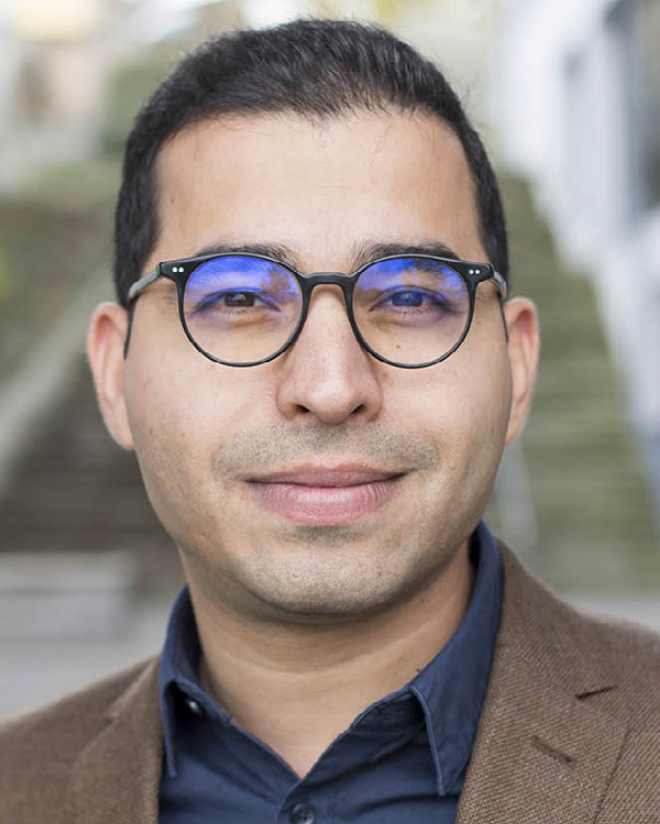
\includegraphics[width=1in,height=1.25in,clip,keepaspectratio]{images/Saleh.PNG}}]{Saleh Javadi} (S'12-M’22) received a B.Sc. degree in electrical-control engineering from Amirkabir University of Technology in 2009, an M.Sc. degree in electrical, electronic, and systems engineering from the National University of Malaysia in 2013, and a Ph.D. degree in systems engineering from Blekinge Institute of Technology (BTH), Sweden, in 2021.

Saleh received the Innovator of the Year award in 2019 (SKAPA – Innovation Prize in Memory of Alfred Nobel) in Blekinge for innovative efforts in optimizing and reducing energy consumption in process industries using artificial intelligence. In addition, he was awarded the ÅForsk Entrepreneur’s prize by the Swedish Innovation Council in May 2019.

He is currently a Senior Lecturer at the Department of Mathematics and Natural Sciences at BTH. His research interests include signal processing, machine learning and computer vision.
\end{IEEEbiography}


\begin{IEEEbiography}[{
\includegraphics[width=1in,height=1.25in,clip,keepaspectratio]{images/Mattias.png}}]{MATTIAS DAHL} 
(Member, IEEE) received a B.Sc.~in Electrical Engineering from Chalmers University of Technology (1989), an M.Sc.~in Computer Science from Luleå University of Technology (1993), a Licentiate degree in Signal Processing from Lund University (1996), and a Ph.D.~in Applied Signal Processing from Blekinge Institute of Technology (2000). Since 2018, he has been a Full Professor at Blekinge Institute of Technology.
His research focuses on autonomous systems, smart sensor systems, applied artificial intelligence (AI), and sustainable engineering. He has led several national and EU-funded research programs and has played a key role in establishing marine technology testbeds, including novel underwater sensing solutions such as Distributed Acoustic Sensing (DAS). He has authored over 120 scientific publications, holds several patents (the latest filed in 2024), and has received innovation awards from Sweden’s Innovation Agency and the Royal Swedish Academy of Engineering Sciences (IVA).
Prof.~Dahl has supervised around 10 Ph.D.~students and is currently supervising three doctoral candidates. His work bridges academia and industry, with contributions in radar, vision, transport systems, and embedded sensing platforms.

\end{IEEEbiography}



\begin{IEEEbiography}[{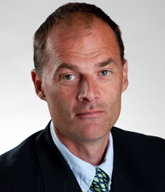
\includegraphics[width=1in,height=1.25in,clip,keepaspectratio]{images/Mats.png}}]{MATS I. PETTERSSON} 
(Senior Member, IEEE) received the M.Sc. in engineering physics, the licentiate degree in radio and space science, and the Ph.D.  in signal processing from the Chalmers University of Technology, Gothenburg, Sweden, in 1993, 1995, and 2000, respectively. 
He worked with Mobile Communication Research at Ericsson, Lund, Sweden. He was with the Swedish Defense Research Agency (FOI) for ten years in Linköping. He focused on ultrawideband low-frequency Synthetic Aperture Radar (SAR) systems at FOI. Since 2005, he has been with the Blekinge Institute of Technology (BTH), Karlskrona, Sweden, where he is a Full Professor. He has authored or co-authored more than 250 scientific publications, of which more than 70 are in peer-reviewed scientific journals. His research is related to radar surveillance and remote sensing. His main research interests include SAR processing, space–time adaptive processing (STAP), high-resolution SAR change detection, automotive radar, radio occultation, THz SAR, and computer vision.
\end{IEEEbiography}




\EOD

\end{document}
